% Options for packages loaded elsewhere
\PassOptionsToPackage{unicode}{hyperref}
\PassOptionsToPackage{hyphens}{url}
\documentclass[
]{article}
\usepackage{xcolor}
\usepackage[margin=1in]{geometry}
\usepackage{amsmath,amssymb}
\setcounter{secnumdepth}{-\maxdimen} % remove section numbering
\usepackage{iftex}
\ifPDFTeX
  \usepackage[T1]{fontenc}
  \usepackage[utf8]{inputenc}
  \usepackage{textcomp} % provide euro and other symbols
\else % if luatex or xetex
  \usepackage{unicode-math} % this also loads fontspec
  \defaultfontfeatures{Scale=MatchLowercase}
  \defaultfontfeatures[\rmfamily]{Ligatures=TeX,Scale=1}
\fi
\usepackage{lmodern}
\ifPDFTeX\else
  % xetex/luatex font selection
\fi
% Use upquote if available, for straight quotes in verbatim environments
\IfFileExists{upquote.sty}{\usepackage{upquote}}{}
\IfFileExists{microtype.sty}{% use microtype if available
  \usepackage[]{microtype}
  \UseMicrotypeSet[protrusion]{basicmath} % disable protrusion for tt fonts
}{}
\makeatletter
\@ifundefined{KOMAClassName}{% if non-KOMA class
  \IfFileExists{parskip.sty}{%
    \usepackage{parskip}
  }{% else
    \setlength{\parindent}{0pt}
    \setlength{\parskip}{6pt plus 2pt minus 1pt}}
}{% if KOMA class
  \KOMAoptions{parskip=half}}
\makeatother
\usepackage{color}
\usepackage{fancyvrb}
\newcommand{\VerbBar}{|}
\newcommand{\VERB}{\Verb[commandchars=\\\{\}]}
\DefineVerbatimEnvironment{Highlighting}{Verbatim}{commandchars=\\\{\}}
% Add ',fontsize=\small' for more characters per line
\usepackage{framed}
\definecolor{shadecolor}{RGB}{248,248,248}
\newenvironment{Shaded}{\begin{snugshade}}{\end{snugshade}}
\newcommand{\AlertTok}[1]{\textcolor[rgb]{0.94,0.16,0.16}{#1}}
\newcommand{\AnnotationTok}[1]{\textcolor[rgb]{0.56,0.35,0.01}{\textbf{\textit{#1}}}}
\newcommand{\AttributeTok}[1]{\textcolor[rgb]{0.13,0.29,0.53}{#1}}
\newcommand{\BaseNTok}[1]{\textcolor[rgb]{0.00,0.00,0.81}{#1}}
\newcommand{\BuiltInTok}[1]{#1}
\newcommand{\CharTok}[1]{\textcolor[rgb]{0.31,0.60,0.02}{#1}}
\newcommand{\CommentTok}[1]{\textcolor[rgb]{0.56,0.35,0.01}{\textit{#1}}}
\newcommand{\CommentVarTok}[1]{\textcolor[rgb]{0.56,0.35,0.01}{\textbf{\textit{#1}}}}
\newcommand{\ConstantTok}[1]{\textcolor[rgb]{0.56,0.35,0.01}{#1}}
\newcommand{\ControlFlowTok}[1]{\textcolor[rgb]{0.13,0.29,0.53}{\textbf{#1}}}
\newcommand{\DataTypeTok}[1]{\textcolor[rgb]{0.13,0.29,0.53}{#1}}
\newcommand{\DecValTok}[1]{\textcolor[rgb]{0.00,0.00,0.81}{#1}}
\newcommand{\DocumentationTok}[1]{\textcolor[rgb]{0.56,0.35,0.01}{\textbf{\textit{#1}}}}
\newcommand{\ErrorTok}[1]{\textcolor[rgb]{0.64,0.00,0.00}{\textbf{#1}}}
\newcommand{\ExtensionTok}[1]{#1}
\newcommand{\FloatTok}[1]{\textcolor[rgb]{0.00,0.00,0.81}{#1}}
\newcommand{\FunctionTok}[1]{\textcolor[rgb]{0.13,0.29,0.53}{\textbf{#1}}}
\newcommand{\ImportTok}[1]{#1}
\newcommand{\InformationTok}[1]{\textcolor[rgb]{0.56,0.35,0.01}{\textbf{\textit{#1}}}}
\newcommand{\KeywordTok}[1]{\textcolor[rgb]{0.13,0.29,0.53}{\textbf{#1}}}
\newcommand{\NormalTok}[1]{#1}
\newcommand{\OperatorTok}[1]{\textcolor[rgb]{0.81,0.36,0.00}{\textbf{#1}}}
\newcommand{\OtherTok}[1]{\textcolor[rgb]{0.56,0.35,0.01}{#1}}
\newcommand{\PreprocessorTok}[1]{\textcolor[rgb]{0.56,0.35,0.01}{\textit{#1}}}
\newcommand{\RegionMarkerTok}[1]{#1}
\newcommand{\SpecialCharTok}[1]{\textcolor[rgb]{0.81,0.36,0.00}{\textbf{#1}}}
\newcommand{\SpecialStringTok}[1]{\textcolor[rgb]{0.31,0.60,0.02}{#1}}
\newcommand{\StringTok}[1]{\textcolor[rgb]{0.31,0.60,0.02}{#1}}
\newcommand{\VariableTok}[1]{\textcolor[rgb]{0.00,0.00,0.00}{#1}}
\newcommand{\VerbatimStringTok}[1]{\textcolor[rgb]{0.31,0.60,0.02}{#1}}
\newcommand{\WarningTok}[1]{\textcolor[rgb]{0.56,0.35,0.01}{\textbf{\textit{#1}}}}
\usepackage{longtable,booktabs,array}
\newcounter{none} % for unnumbered tables
\usepackage{calc} % for calculating minipage widths
% Correct order of tables after \paragraph or \subparagraph
\usepackage{etoolbox}
\makeatletter
\patchcmd\longtable{\par}{\if@noskipsec\mbox{}\fi\par}{}{}
\makeatother
% Allow footnotes in longtable head/foot
\IfFileExists{footnotehyper.sty}{\usepackage{footnotehyper}}{\usepackage{footnote}}
\makesavenoteenv{longtable}
\usepackage{graphicx}
\makeatletter
\newsavebox\pandoc@box
\newcommand*\pandocbounded[1]{% scales image to fit in text height/width
  \sbox\pandoc@box{#1}%
  \Gscale@div\@tempa{\textheight}{\dimexpr\ht\pandoc@box+\dp\pandoc@box\relax}%
  \Gscale@div\@tempb{\linewidth}{\wd\pandoc@box}%
  \ifdim\@tempb\p@<\@tempa\p@\let\@tempa\@tempb\fi% select the smaller of both
  \ifdim\@tempa\p@<\p@\scalebox{\@tempa}{\usebox\pandoc@box}%
  \else\usebox{\pandoc@box}%
  \fi%
}
% Set default figure placement to htbp
\def\fps@figure{htbp}
\makeatother
\setlength{\emergencystretch}{3em} % prevent overfull lines
\providecommand{\tightlist}{%
  \setlength{\itemsep}{0pt}\setlength{\parskip}{0pt}}
\usepackage{bookmark}
\IfFileExists{xurl.sty}{\usepackage{xurl}}{} % add URL line breaks if available
\urlstyle{same}
% fallback for those not using the hyperref driver hyperxmp:
\makeatletter
\@ifundefined{xmpquote}{\newcommand{\xmpquote}[1]{#1}}{}
\makeatother
\hypersetup{
  pdftitle={2026-10-05\_p8157\_hw-01},
  pdfauthor={Chris},
  hidelinks,
  pdfcreator={LaTeX via pandoc}}

\title{2026-10-05\_p8157\_hw-01}
\author{Chris}
\date{2026-10-05}

\begin{document}
\maketitle

\textbf{Acknowledgement}: The author would like to acknowledge the use
of ChatGPT, a language model developed by OpenAI, in the preparation of
this assignment. ChatGPT was used in the following ways in this
assignment:\\
* Helping me organize the codes for generating Table One.\\
* Providing a detailed mind map for EDA.\\
* Suggesting me add more security checks.\\
* Helping to make the plots more human-friendly.

The full homework can be found here:
\url{https://github.com/ChrisW12372/2026-10-05_p8157_hw-01.git}

\begin{Shaded}
\begin{Highlighting}[]
\FunctionTok{library}\NormalTok{(tidyverse)}
\FunctionTok{library}\NormalTok{(lme4)}
\FunctionTok{library}\NormalTok{(plotly)}
\FunctionTok{library}\NormalTok{(knitr)}
\FunctionTok{library}\NormalTok{(splines)}
\FunctionTok{library}\NormalTok{(broom)}

\FunctionTok{load}\NormalTok{(}\StringTok{"data/Six Cities.RData"}\NormalTok{)}
\FunctionTok{load}\NormalTok{(}\StringTok{"data/MACS.RData"}\NormalTok{)}
\end{Highlighting}
\end{Shaded}

\section{Question 2}\label{question-2}

\subsection{EDA for topeka}\label{eda-for-topeka}

\subsubsection{overall checking}\label{overall-checking}

\begin{Shaded}
\begin{Highlighting}[]
\NormalTok{df\_topeka }\OtherTok{\textless{}{-}}\NormalTok{ topeka }\SpecialCharTok{|\textgreater{}}
  \FunctionTok{arrange}\NormalTok{(id, age) }\SpecialCharTok{|\textgreater{}}
  \FunctionTok{mutate}\NormalTok{(}
    \AttributeTok{height =} \FunctionTok{as.numeric}\NormalTok{(height),}
    \AttributeTok{age =} \FunctionTok{as.numeric}\NormalTok{(age),}
    \AttributeTok{height.init =} \FunctionTok{as.numeric}\NormalTok{(height.init),}
    \AttributeTok{age.init =} \FunctionTok{as.numeric}\NormalTok{(age.init)}
\NormalTok{  )}
\end{Highlighting}
\end{Shaded}

\begin{Shaded}
\begin{Highlighting}[]
\NormalTok{df\_topeka\_summary }\OtherTok{\textless{}{-}}\NormalTok{ df\_topeka }\SpecialCharTok{|\textgreater{}}
  \FunctionTok{group\_by}\NormalTok{(id) }\SpecialCharTok{|\textgreater{}}
  \FunctionTok{summarise}\NormalTok{(}
    \AttributeTok{n\_visits =} \FunctionTok{n}\NormalTok{(),}
    \AttributeTok{age\_first =} \FunctionTok{first}\NormalTok{(age),}
    \AttributeTok{age\_last =} \FunctionTok{last}\NormalTok{(age),}
    \AttributeTok{follow\_up\_time =}\NormalTok{ age\_last }\SpecialCharTok{{-}}\NormalTok{ age\_first,}
    \AttributeTok{height\_fitst =} \FunctionTok{first}\NormalTok{(height),}
    \AttributeTok{log\_fev1\_first =} \FunctionTok{first}\NormalTok{(log.FEV1),}
    \AttributeTok{.groups =} \StringTok{"drop"}
\NormalTok{  )}

\FunctionTok{write\_csv}\NormalTok{(df\_topeka\_summary, }\StringTok{"results/2026{-}10{-}05\_topeka{-}summary.csv"}\NormalTok{)}
\end{Highlighting}
\end{Shaded}

\begin{Shaded}
\begin{Highlighting}[]
\CommentTok{\# check for NA}
\FunctionTok{colSums}\NormalTok{(}\FunctionTok{is.na}\NormalTok{(df\_topeka))}
\end{Highlighting}
\end{Shaded}

\begin{verbatim}
##          id      height         age height.init    age.init    log.FEV1 
##           0           0           0           0           0           0
\end{verbatim}

\begin{Shaded}
\begin{Highlighting}[]
\CommentTok{\# check for duplicated values within one age}
\NormalTok{df\_topeka }\SpecialCharTok{|\textgreater{}}
  \FunctionTok{count}\NormalTok{(id, age, }\AttributeTok{name =} \StringTok{"n\_records"}\NormalTok{) }\SpecialCharTok{|\textgreater{}}
  \FunctionTok{filter}\NormalTok{(n\_records }\SpecialCharTok{\textgreater{}} \DecValTok{1}\NormalTok{)}
\end{Highlighting}
\end{Shaded}

\begin{verbatim}
## [1] id        age       n_records
## <0 rows> (or 0-length row.names)
\end{verbatim}

\begin{Shaded}
\begin{Highlighting}[]
\CommentTok{\# non{-}positive follow{-}up time}
\NormalTok{df\_one\_visit }\OtherTok{\textless{}{-}} 
\NormalTok{  df\_topeka\_summary }\SpecialCharTok{|\textgreater{}}
  \FunctionTok{filter}\NormalTok{(follow\_up\_time }\SpecialCharTok{\textless{}=} \DecValTok{0}\NormalTok{)}

\FunctionTok{write\_csv}\NormalTok{(df\_one\_visit, }\StringTok{"results/2026{-}10{-}05\_topeka\_subjects{-}one{-}visit.csv"}\NormalTok{)}

\CommentTok{\# whether the first measurements of age and height match the initial values }
\NormalTok{df\_baseline\_check }\OtherTok{\textless{}{-}} 
\NormalTok{  df\_topeka }\SpecialCharTok{|\textgreater{}}
  \FunctionTok{group\_by}\NormalTok{(id) }\SpecialCharTok{|\textgreater{}}
  \FunctionTok{summarise}\NormalTok{(}
    \AttributeTok{age\_init\_match =} \FunctionTok{all}\NormalTok{(}\FunctionTok{abs}\NormalTok{(}\FunctionTok{first}\NormalTok{(age) }\SpecialCharTok{{-}}\NormalTok{ age.init) }\SpecialCharTok{==} \DecValTok{0}\NormalTok{),}
    \AttributeTok{height\_init\_match =} \FunctionTok{all}\NormalTok{(}\FunctionTok{abs}\NormalTok{(}\FunctionTok{first}\NormalTok{(height) }\SpecialCharTok{{-}}\NormalTok{ height.init) }\SpecialCharTok{==} \DecValTok{0}\NormalTok{),}
    \AttributeTok{.groups =} \StringTok{"drop"}
\NormalTok{  )}

\FunctionTok{write\_csv}\NormalTok{(df\_baseline\_check, }\StringTok{"results/2026{-}10{-}05\_topeka\_baseline{-}match.csv"}\NormalTok{)}
\end{Highlighting}
\end{Shaded}

\begin{Shaded}
\begin{Highlighting}[]
\NormalTok{describe\_row }\OtherTok{\textless{}{-}} \ControlFlowTok{function}\NormalTok{(label, x) \{}
\NormalTok{  x }\OtherTok{\textless{}{-}}\NormalTok{ x[}\SpecialCharTok{!}\FunctionTok{is.na}\NormalTok{(x)]}

  \FunctionTok{tibble}\NormalTok{(}
    \AttributeTok{Characteristic =}\NormalTok{ label,}
    \AttributeTok{N =} \FunctionTok{length}\NormalTok{(x),}
    \StringTok{\textasciigrave{}}\AttributeTok{Mean (SD)}\StringTok{\textasciigrave{}} \OtherTok{=} \FunctionTok{sprintf}\NormalTok{(}
      \StringTok{"\%.2f (\%.2f)"}\NormalTok{, }\FunctionTok{mean}\NormalTok{(x), }\FunctionTok{sd}\NormalTok{(x)}
\NormalTok{    ),}
    \StringTok{\textasciigrave{}}\AttributeTok{Median [Q1, Q3]}\StringTok{\textasciigrave{}} \OtherTok{=} \FunctionTok{sprintf}\NormalTok{(}
      \StringTok{"\%.2f [\%.2f, \%.2f]"}\NormalTok{,}
      \FunctionTok{median}\NormalTok{(x),}
      \FunctionTok{quantile}\NormalTok{(x, }\FloatTok{0.25}\NormalTok{),}
      \FunctionTok{quantile}\NormalTok{(x, }\FloatTok{0.75}\NormalTok{)}
\NormalTok{    ),}
    \StringTok{\textasciigrave{}}\AttributeTok{Min–Max}\StringTok{\textasciigrave{}} \OtherTok{=} \FunctionTok{sprintf}\NormalTok{(}
      \StringTok{"\%.2f–\%.2f"}\NormalTok{, }\FunctionTok{min}\NormalTok{(x), }\FunctionTok{max}\NormalTok{(x)}
\NormalTok{    )}
\NormalTok{  )}
\NormalTok{\}}
\end{Highlighting}
\end{Shaded}

\begin{Shaded}
\begin{Highlighting}[]
\NormalTok{overview\_table }\OtherTok{\textless{}{-}} \FunctionTok{bind\_rows}\NormalTok{(}
  \FunctionTok{describe\_row}\NormalTok{(}
    \StringTok{"Measurements per girl"}\NormalTok{,}
\NormalTok{    df\_topeka\_summary}\SpecialCharTok{$}\NormalTok{n\_visits}
\NormalTok{  ),}
  \FunctionTok{describe\_row}\NormalTok{(}
    \StringTok{"Age at first observation (years)"}\NormalTok{,}
\NormalTok{    df\_topeka\_summary}\SpecialCharTok{$}\NormalTok{age\_first}
\NormalTok{  ),}
  \FunctionTok{describe\_row}\NormalTok{(}
    \StringTok{"Age at last observation (years)"}\NormalTok{,}
\NormalTok{    df\_topeka\_summary}\SpecialCharTok{$}\NormalTok{age\_last}
\NormalTok{  ),}
  \FunctionTok{describe\_row}\NormalTok{(}
    \StringTok{"Observed follow{-}up span (years)"}\NormalTok{,}
\NormalTok{    df\_topeka\_summary}\SpecialCharTok{$}\NormalTok{follow\_up\_time}
\NormalTok{  ),}
  \FunctionTok{describe\_row}\NormalTok{(}
    \StringTok{"Height at first observation"}\NormalTok{,}
\NormalTok{    df\_topeka\_summary}\SpecialCharTok{$}\NormalTok{height\_fitst}
\NormalTok{  ),}
  \FunctionTok{describe\_row}\NormalTok{(}
    \StringTok{"Log(FEV1) at first observation"}\NormalTok{,}
\NormalTok{    df\_topeka\_summary}\SpecialCharTok{$}\NormalTok{log\_fev1\_first}
\NormalTok{  ),}
  \FunctionTok{describe\_row}\NormalTok{(}
    \StringTok{"Age across all observations (years)"}\NormalTok{,}
\NormalTok{    df\_topeka}\SpecialCharTok{$}\NormalTok{age}
\NormalTok{  ),}
  \FunctionTok{describe\_row}\NormalTok{(}
    \StringTok{"Height across all observations"}\NormalTok{,}
\NormalTok{    df\_topeka}\SpecialCharTok{$}\NormalTok{height}
\NormalTok{  ),}
  \FunctionTok{describe\_row}\NormalTok{(}
    \StringTok{"Log(FEV1) across all observations"}\NormalTok{,}
\NormalTok{    df\_topeka}\SpecialCharTok{$}\NormalTok{log.FEV1}
\NormalTok{  )}
\NormalTok{)}

\FunctionTok{kable}\NormalTok{(}
\NormalTok{  overview\_table,}
  \AttributeTok{caption =} \StringTok{"Table 1. Data and follow{-}up characteristics of the Topeka sample"}\NormalTok{,}
  \AttributeTok{col.names =} \FunctionTok{c}\NormalTok{(}
    \StringTok{"Characteristic"}\NormalTok{,}
    \StringTok{"N"}\NormalTok{,}
    \StringTok{"Mean (SD)"}\NormalTok{,}
    \StringTok{"Median [Q1, Q3]"}\NormalTok{,}
    \StringTok{"Min–Max"}
\NormalTok{  ),}
  \AttributeTok{align =} \FunctionTok{c}\NormalTok{(}\StringTok{"l"}\NormalTok{, }\StringTok{"r"}\NormalTok{, }\StringTok{"r"}\NormalTok{, }\StringTok{"r"}\NormalTok{, }\StringTok{"r"}\NormalTok{),}
  \AttributeTok{row.names =} \ConstantTok{FALSE}
\NormalTok{)}
\end{Highlighting}
\end{Shaded}

\begin{longtable}[]{@{}
  >{\raggedright\arraybackslash}p{(\linewidth - 8\tabcolsep) * \real{0.4186}}
  >{\raggedleft\arraybackslash}p{(\linewidth - 8\tabcolsep) * \real{0.0581}}
  >{\raggedleft\arraybackslash}p{(\linewidth - 8\tabcolsep) * \real{0.1512}}
  >{\raggedleft\arraybackslash}p{(\linewidth - 8\tabcolsep) * \real{0.2442}}
  >{\raggedleft\arraybackslash}p{(\linewidth - 8\tabcolsep) * \real{0.1279}}@{}}
\caption{Table 1. Data and follow-up characteristics of the Topeka
sample}\tabularnewline
\toprule\noalign{}
\begin{minipage}[b]{\linewidth}\raggedright
Characteristic
\end{minipage} & \begin{minipage}[b]{\linewidth}\raggedleft
N
\end{minipage} & \begin{minipage}[b]{\linewidth}\raggedleft
Mean (SD)
\end{minipage} & \begin{minipage}[b]{\linewidth}\raggedleft
Median {[}Q1, Q3{]}
\end{minipage} & \begin{minipage}[b]{\linewidth}\raggedleft
Min--Max
\end{minipage} \\
\midrule\noalign{}
\endfirsthead
\toprule\noalign{}
\begin{minipage}[b]{\linewidth}\raggedright
Characteristic
\end{minipage} & \begin{minipage}[b]{\linewidth}\raggedleft
N
\end{minipage} & \begin{minipage}[b]{\linewidth}\raggedleft
Mean (SD)
\end{minipage} & \begin{minipage}[b]{\linewidth}\raggedleft
Median {[}Q1, Q3{]}
\end{minipage} & \begin{minipage}[b]{\linewidth}\raggedleft
Min--Max
\end{minipage} \\
\midrule\noalign{}
\endhead
\bottomrule\noalign{}
\endlastfoot
Measurements per girl & 300 & 6.65 (3.85) & 7.00 {[}3.00, 10.00{]} &
1.00--12.00 \\
Age at first observation (years) & 300 & 8.30 (1.38) & 8.02 {[}7.33,
8.95{]} & 6.43--14.07 \\
Age at last observation (years) & 300 & 14.98 (3.84) & 17.25 {[}11.68,
17.99{]} & 6.66--18.69 \\
Observed follow-up span (years) & 300 & 6.69 (4.12) & 8.08 {[}2.02,
10.03{]} & 0.00--11.06 \\
Height at first observation & 300 & 1.29 (0.10) & 1.27 {[}1.22, 1.34{]}
& 1.11--1.72 \\
Log(FEV1) at first observation & 300 & 0.38 (0.22) & 0.36 {[}0.24,
0.50{]} & -0.69--1.37 \\
Age across all observations (years) & 1994 & 12.57 (3.32) & 12.60
{[}9.72, 15.37{]} & 6.43--18.69 \\
Height across all observations & 1994 & 1.50 (0.15) & 1.54 {[}1.37,
1.62{]} & 1.11--1.79 \\
Log(FEV1) across all observations & 1994 & 0.82 (0.33) & 0.87 {[}0.55,
1.10{]} & -0.69--1.60 \\
\end{longtable}

The data include 1,994 measurements from 300 girls. Each girl has 1--12
measurements, and 48 girls (16\%) have only one. I will keep all girls
in the analysis and use a model that can handle different numbers of
measurements. Girls with only one measurement can help estimate average
lung function, but cannot show how it changes within a person.

Girls were first observed at different ages, from 6.43 to 14.07 years. I
will use actual age rather than visit number to study lung growth. I
will also check how many observations are available at each age and
whether girls with shorter follow-up differ from those with longer
follow-up.

Initial age and height match the first recorded values for all girls.
The lowest log(FEV1) is about −0.69. I will check this value against the
girl's age and height before deciding whether it is unusual.

\subsubsection{mean structure}\label{mean-structure}

\paragraph{age \textasciitilde{} log(FEV1)}\label{age-logfev1}

\begin{Shaded}
\begin{Highlighting}[]
\NormalTok{fig1\_topeka\_spaghetti }\OtherTok{\textless{}{-}} 
\NormalTok{  df\_topeka }\SpecialCharTok{|\textgreater{}}
  \FunctionTok{ggplot}\NormalTok{(}\FunctionTok{aes}\NormalTok{(}\AttributeTok{x =}\NormalTok{ age, }\AttributeTok{y =}\NormalTok{ log.FEV1)) }\SpecialCharTok{+}
  \FunctionTok{geom\_line}\NormalTok{(}\FunctionTok{aes}\NormalTok{(}\AttributeTok{group =}\NormalTok{ id), }\AttributeTok{color =} \StringTok{"\#32BFAD"}\NormalTok{, }\AttributeTok{alpha =} \FloatTok{0.25}\NormalTok{, }\AttributeTok{linewidth =} \FloatTok{0.4}\NormalTok{) }\SpecialCharTok{+}
  \FunctionTok{geom\_point}\NormalTok{(}\AttributeTok{color =} \StringTok{"\#3810A3"}\NormalTok{, }\AttributeTok{alpha =} \FloatTok{0.25}\NormalTok{, }\AttributeTok{size =} \FloatTok{0.75}\NormalTok{) }\SpecialCharTok{+}
  \FunctionTok{geom\_smooth}\NormalTok{(}\AttributeTok{method =} \StringTok{"loess"}\NormalTok{, }\AttributeTok{formula =}\NormalTok{ y }\SpecialCharTok{\textasciitilde{}}\NormalTok{ x, }\AttributeTok{se =} \ConstantTok{FALSE}\NormalTok{, }\AttributeTok{color =} \StringTok{"\#0072B2"}\NormalTok{) }\SpecialCharTok{+}
  \FunctionTok{labs}\NormalTok{(}
    \AttributeTok{title =} \StringTok{"Lung function trajectories"}\NormalTok{,}
    \AttributeTok{x =} \StringTok{"Age (years)"}\NormalTok{,}
    \AttributeTok{y =} \StringTok{"Log(FEV1)"}
\NormalTok{  ) }\SpecialCharTok{+} \FunctionTok{theme\_minimal}\NormalTok{()}

\FunctionTok{ggsave}\NormalTok{(}\StringTok{"plots/2026{-}10{-}05\_fig01\_topeka\_spaghetti{-}plot.png"}\NormalTok{, fig1\_topeka\_spaghetti,}
       \AttributeTok{height =} \DecValTok{6}\NormalTok{, }\AttributeTok{width =} \DecValTok{9}\NormalTok{, }\AttributeTok{dpi =} \DecValTok{1000}\NormalTok{)}

\NormalTok{fig1\_topeka\_spaghetti}
\end{Highlighting}
\end{Shaded}

\pandocbounded{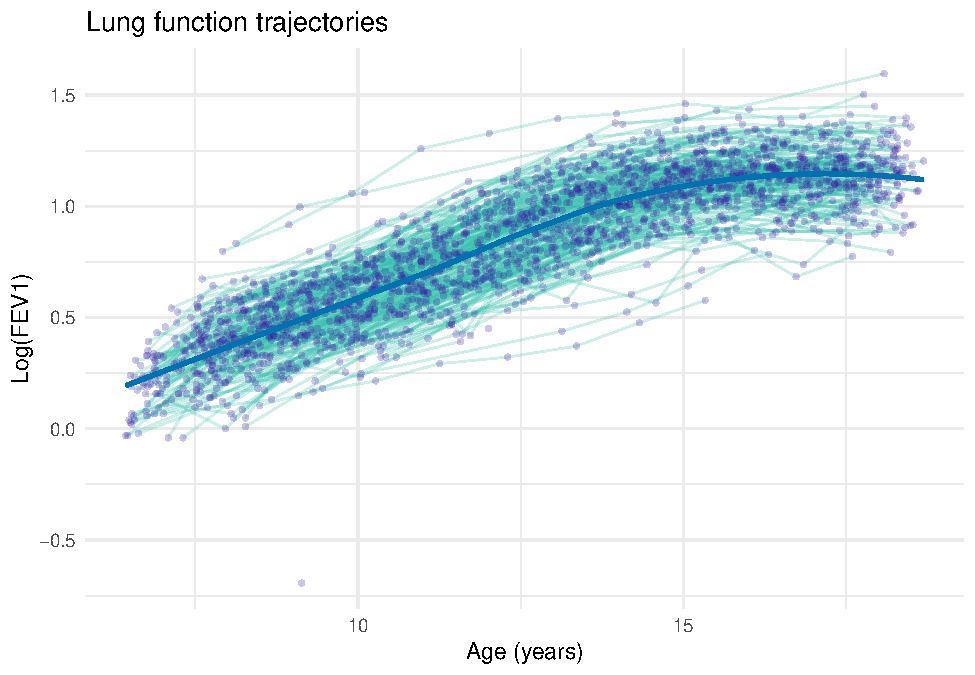
\includegraphics[keepaspectratio]{2026-10-05_p8157_hw-01_knit-to-pdf_files/figure-latex/unnamed-chunk-7-1.pdf}}

\begin{Shaded}
\begin{Highlighting}[]
\CommentTok{\# find out the outlier}
\NormalTok{outlier\_topeka }\OtherTok{\textless{}{-}}\NormalTok{ df\_topeka }\SpecialCharTok{|\textgreater{}}
  \FunctionTok{slice\_min}\NormalTok{(log.FEV1, }\AttributeTok{n =} \DecValTok{1}\NormalTok{, }\AttributeTok{with\_ties =} \ConstantTok{TRUE}\NormalTok{)}

\NormalTok{outlier\_topeka}
\end{Highlighting}
\end{Shaded}

\begin{verbatim}
##    id height    age height.init age.init log.FEV1
## 1 197   1.22 9.1362        1.22   9.1362 -0.69315
\end{verbatim}

\begin{Shaded}
\begin{Highlighting}[]
\CommentTok{\# checking all measurements of id 197}
\NormalTok{df\_topeka }\SpecialCharTok{|\textgreater{}}
  \FunctionTok{filter}\NormalTok{(id }\SpecialCharTok{==} \DecValTok{197}\NormalTok{) }\SpecialCharTok{|\textgreater{}}
  \FunctionTok{arrange}\NormalTok{(id, age)}
\end{Highlighting}
\end{Shaded}

\begin{verbatim}
##    id height    age height.init age.init log.FEV1
## 1 197   1.22 9.1362        1.22   9.1362 -0.69315
\end{verbatim}

Log(FEV1) generally increases with age and levels off around ages
15--16. I will therefore consider a nonlinear age effect in later
models. Lung function also differs across girls, so I will explore
within-person correlation.

Subject 197 has a clearly low value and only one measurement, so I
cannot compare it with her other visits. I will retain this observation
for now, and later decide whether to include it into the analysis.

\paragraph{height \textasciitilde{} log(FEV1)}\label{height-logfev1}

\begin{Shaded}
\begin{Highlighting}[]
\NormalTok{fig2\_topeka\_points }\OtherTok{\textless{}{-}} 
\NormalTok{  df\_topeka }\SpecialCharTok{|\textgreater{}}
  \FunctionTok{ggplot}\NormalTok{(}\FunctionTok{aes}\NormalTok{(}\AttributeTok{x =}\NormalTok{ height, }\AttributeTok{y =}\NormalTok{ log.FEV1)) }\SpecialCharTok{+}
  \FunctionTok{geom\_point}\NormalTok{(}\AttributeTok{color =} \StringTok{"\#DB662C"}\NormalTok{, }\AttributeTok{alpha =} \FloatTok{0.35}\NormalTok{, }\AttributeTok{size =} \FloatTok{0.75}\NormalTok{) }\SpecialCharTok{+}
  \FunctionTok{geom\_smooth}\NormalTok{(}\AttributeTok{method =} \StringTok{"loess"}\NormalTok{, }\AttributeTok{formula =}\NormalTok{ y }\SpecialCharTok{\textasciitilde{}}\NormalTok{ x, }\AttributeTok{se =} \ConstantTok{FALSE}\NormalTok{, }\AttributeTok{colour =} \StringTok{"\#8A2278"}\NormalTok{) }\SpecialCharTok{+}
  \FunctionTok{geom\_point}\NormalTok{(}\AttributeTok{data =}\NormalTok{ outlier\_topeka, }\AttributeTok{colour =} \StringTok{"\#5a6acd"}\NormalTok{) }\SpecialCharTok{+}
  \FunctionTok{geom\_text}\NormalTok{(}\AttributeTok{data =}\NormalTok{ outlier\_topeka, }\AttributeTok{colour =} \StringTok{"\#E6DD39"}\NormalTok{, }\FunctionTok{aes}\NormalTok{(}\AttributeTok{label =} \FunctionTok{paste0}\NormalTok{(}\StringTok{"ID"}\NormalTok{, id)), }\AttributeTok{vjust =} \SpecialCharTok{{-}}\DecValTok{1}\NormalTok{) }\SpecialCharTok{+}
  \FunctionTok{labs}\NormalTok{(}
    \AttributeTok{title =} \StringTok{"Lung function and height"}\NormalTok{,}
    \AttributeTok{x =} \StringTok{"Height"}\NormalTok{,}
    \AttributeTok{y =} \StringTok{"Log(FEV1)"}
\NormalTok{  ) }\SpecialCharTok{+} \FunctionTok{theme\_minimal}\NormalTok{()}

\FunctionTok{ggsave}\NormalTok{(}\StringTok{"plots/2026{-}10{-}05\_fig02\_topeka\_point{-}plot.png"}\NormalTok{, fig2\_topeka\_points,}
       \AttributeTok{height =} \DecValTok{6}\NormalTok{, }\AttributeTok{width =} \DecValTok{9}\NormalTok{, }\AttributeTok{dpi =} \DecValTok{1200}\NormalTok{)}

\NormalTok{fig2\_topeka\_points}
\end{Highlighting}
\end{Shaded}

\pandocbounded{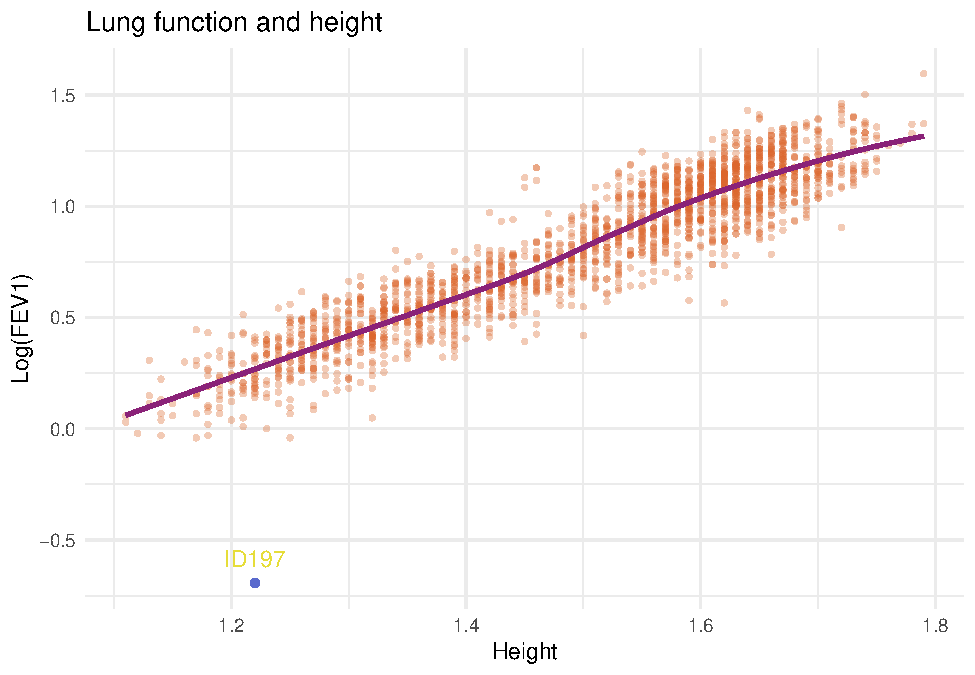
\includegraphics[keepaspectratio]{2026-10-05_p8157_hw-01_knit-to-pdf_files/figure-latex/unnamed-chunk-10-1.pdf}}

Log(FEV1) increases with height, and the relationship is roughly linear.
I will include height in the mean model and compare a linear height
effect with a more flexible form. Subject 197 also has unusually low
lung function compared with girls of similar height.

\paragraph{age \textasciitilde{} height}\label{age-height}

\begin{Shaded}
\begin{Highlighting}[]
\NormalTok{fig3\_topeka\_age\_height\_spaghetti }\OtherTok{\textless{}{-}} 
\NormalTok{  df\_topeka }\SpecialCharTok{|\textgreater{}}
  \FunctionTok{ggplot}\NormalTok{(}\FunctionTok{aes}\NormalTok{(}\AttributeTok{x =}\NormalTok{ age, }\AttributeTok{y =}\NormalTok{ height)) }\SpecialCharTok{+}
  \FunctionTok{geom\_line}\NormalTok{(}\FunctionTok{aes}\NormalTok{(}\AttributeTok{group =}\NormalTok{ id), }\AttributeTok{color =} \StringTok{"\#7FBA38"}\NormalTok{, }\AttributeTok{alpha =} \FloatTok{0.25}\NormalTok{, }\AttributeTok{linewidth =} \FloatTok{0.4}\NormalTok{) }\SpecialCharTok{+}
  \FunctionTok{geom\_point}\NormalTok{(}\AttributeTok{color =} \StringTok{"\#6EAFDB"}\NormalTok{, }\AttributeTok{alpha =} \FloatTok{0.35}\NormalTok{) }\SpecialCharTok{+}
  \FunctionTok{geom\_smooth}\NormalTok{(}\AttributeTok{method =} \StringTok{"loess"}\NormalTok{, }\AttributeTok{formula =}\NormalTok{ y }\SpecialCharTok{\textasciitilde{}}\NormalTok{ x, }\AttributeTok{se =} \ConstantTok{FALSE}\NormalTok{, }\AttributeTok{color =} \StringTok{"\#894CC7"}\NormalTok{) }\SpecialCharTok{+}
  \FunctionTok{labs}\NormalTok{(}
    \AttributeTok{title =} \StringTok{"Height trajectories"}\NormalTok{,}
    \AttributeTok{x =} \StringTok{"Age (years)"}\NormalTok{,}
    \AttributeTok{y =} \StringTok{"Height"}
\NormalTok{  ) }\SpecialCharTok{+} \FunctionTok{theme\_minimal}\NormalTok{()}

\FunctionTok{ggsave}\NormalTok{(}\StringTok{"plots/2026{-}10{-}05\_fig03\_topeka\_age{-}height{-}spaghetti.png"}\NormalTok{, fig3\_topeka\_age\_height\_spaghetti, }\AttributeTok{height =} \DecValTok{6}\NormalTok{, }\AttributeTok{width =} \DecValTok{9}\NormalTok{, }\AttributeTok{dpi =} \DecValTok{1000}\NormalTok{)}

\NormalTok{fig3\_topeka\_age\_height\_spaghetti}
\end{Highlighting}
\end{Shaded}

\pandocbounded{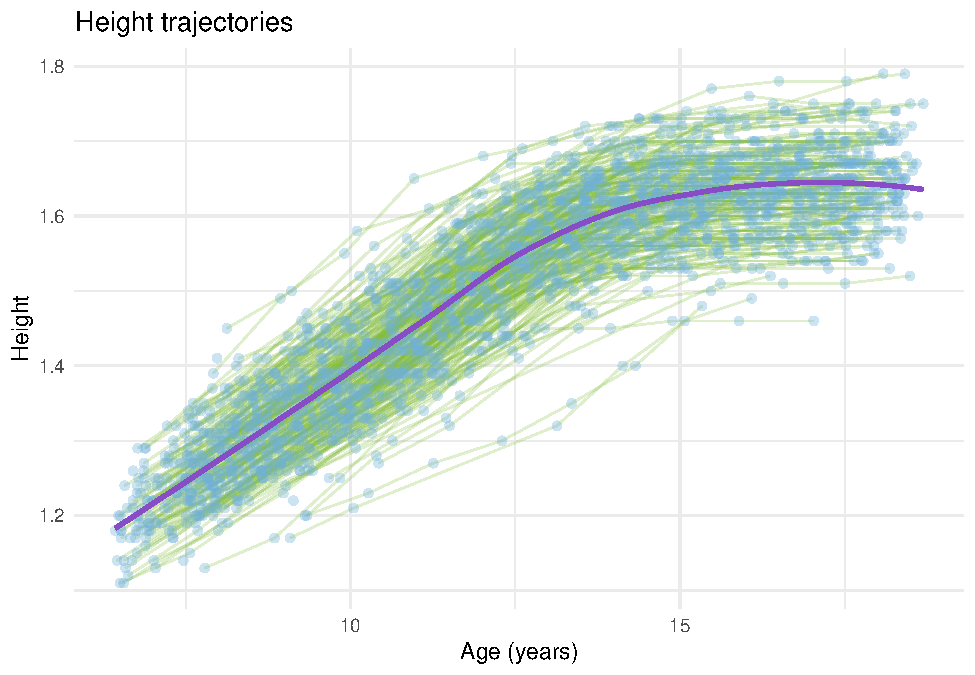
\includegraphics[keepaspectratio]{2026-10-05_p8157_hw-01_knit-to-pdf_files/figure-latex/unnamed-chunk-11-1.pdf}}

Height increases with age and levels off in the teenage years. Since age
and height are closely related, I will interpret their effects carefully
when both are included in the model. The age effect after adjusting for
height describes differences between girls of the same height, rather
than the overall age-related growth pattern.

\subsubsection{dependence structure}\label{dependence-structure}

\begin{Shaded}
\begin{Highlighting}[]
\NormalTok{mean\_fit }\OtherTok{\textless{}{-}} \FunctionTok{lm}\NormalTok{(log.FEV1 }\SpecialCharTok{\textasciitilde{}} \FunctionTok{ns}\NormalTok{(age, }\AttributeTok{df =} \DecValTok{3}\NormalTok{) }\SpecialCharTok{+} \FunctionTok{ns}\NormalTok{(height, }\AttributeTok{df =} \DecValTok{3}\NormalTok{), }\AttributeTok{data =}\NormalTok{ df\_topeka)}

\NormalTok{df\_topeka}\SpecialCharTok{$}\NormalTok{residual\_mean }\OtherTok{\textless{}{-}} \FunctionTok{residuals}\NormalTok{(mean\_fit)}
\end{Highlighting}
\end{Shaded}

\begin{Shaded}
\begin{Highlighting}[]
\NormalTok{fig4\_topeka\_residuals\_spline }\OtherTok{\textless{}{-}} 
\NormalTok{  df\_topeka }\SpecialCharTok{|\textgreater{}}
  \FunctionTok{ggplot}\NormalTok{(}\FunctionTok{aes}\NormalTok{(}\AttributeTok{x =}\NormalTok{ age, }\AttributeTok{y =}\NormalTok{ residual\_mean)) }\SpecialCharTok{+}
    \FunctionTok{geom\_line}\NormalTok{(}
      \FunctionTok{aes}\NormalTok{(}\AttributeTok{group =}\NormalTok{ id),}
      \AttributeTok{color =} \StringTok{"\#559E9E"}\NormalTok{,}
      \AttributeTok{alpha =} \FloatTok{0.25}\NormalTok{,}
      \AttributeTok{linewidth =} \FloatTok{0.4}
\NormalTok{    ) }\SpecialCharTok{+}
    \FunctionTok{geom\_point}\NormalTok{(}\AttributeTok{alpha =} \FloatTok{0.25}\NormalTok{, }\AttributeTok{size =} \FloatTok{0.8}\NormalTok{) }\SpecialCharTok{+}
    \FunctionTok{geom\_smooth}\NormalTok{(}
      \AttributeTok{method =} \StringTok{"loess"}\NormalTok{,}
      \AttributeTok{formula =}\NormalTok{ y }\SpecialCharTok{\textasciitilde{}}\NormalTok{ x,}
      \AttributeTok{se =} \ConstantTok{FALSE}\NormalTok{,}
      \AttributeTok{color =} \StringTok{"\#0072B2"}
\NormalTok{    ) }\SpecialCharTok{+}
    \FunctionTok{labs}\NormalTok{(}
      \AttributeTok{title =} \StringTok{"Residual lung function trajectories"}\NormalTok{,}
      \AttributeTok{x =} \StringTok{"Age (years)"}\NormalTok{,}
      \AttributeTok{y =} \StringTok{"Residual log(FEV1)"}
\NormalTok{    ) }\SpecialCharTok{+} \FunctionTok{theme\_minimal}\NormalTok{()}

\FunctionTok{ggsave}\NormalTok{(}\StringTok{"plots/2026{-}10{-}05\_fig04\_topeka\_residual{-}plot\_splines.png"}\NormalTok{,}
\NormalTok{       fig4\_topeka\_residuals\_spline, }\AttributeTok{height =} \DecValTok{6}\NormalTok{, }\AttributeTok{width =} \DecValTok{9}\NormalTok{, }\AttributeTok{dpi =} \DecValTok{900}\NormalTok{)}

\NormalTok{fig4\_topeka\_residuals\_spline}
\end{Highlighting}
\end{Shaded}

\pandocbounded{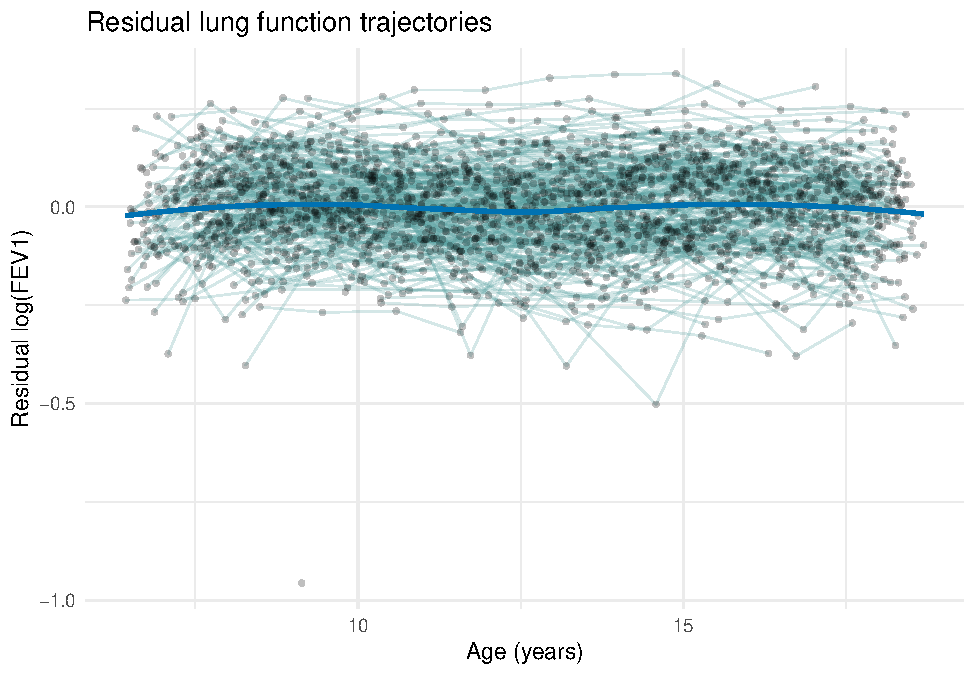
\includegraphics[keepaspectratio]{2026-10-05_p8157_hw-01_knit-to-pdf_files/figure-latex/unnamed-chunk-13-1.pdf}}

The residual smooth is close to zero, with no clear remaining age trend.
Some girls have residuals that stay above or below zero across visits,
suggesting persistent differences between girls. I will consider a
random intercept to capture these differences and use the variogram to
explore whether correlation also changes with the time gap.

\begin{Shaded}
\begin{Highlighting}[]
\NormalTok{pair\_data }\OtherTok{\textless{}{-}} \FunctionTok{bind\_rows}\NormalTok{(}
  \FunctionTok{lapply}\NormalTok{(}\FunctionTok{split}\NormalTok{(df\_topeka, df\_topeka}\SpecialCharTok{$}\NormalTok{id), }\ControlFlowTok{function}\NormalTok{(d) \{}

\NormalTok{    d }\OtherTok{\textless{}{-}}\NormalTok{ d }\SpecialCharTok{\%\textgreater{}\%}
      \FunctionTok{filter}\NormalTok{(}\FunctionTok{is.finite}\NormalTok{(age), }\FunctionTok{is.finite}\NormalTok{(residual\_mean)) }\SpecialCharTok{|\textgreater{}}
      \FunctionTok{arrange}\NormalTok{(age)}

    \ControlFlowTok{if}\NormalTok{ (}\FunctionTok{nrow}\NormalTok{(d) }\SpecialCharTok{\textless{}} \DecValTok{2}\NormalTok{) }\FunctionTok{return}\NormalTok{(}\ConstantTok{NULL}\NormalTok{)}

\NormalTok{    index }\OtherTok{\textless{}{-}} \FunctionTok{combn}\NormalTok{(}\FunctionTok{seq\_len}\NormalTok{(}\FunctionTok{nrow}\NormalTok{(d)), }\DecValTok{2}\NormalTok{)}
\NormalTok{    j }\OtherTok{\textless{}{-}}\NormalTok{ index[}\DecValTok{1}\NormalTok{, ]}
\NormalTok{    k }\OtherTok{\textless{}{-}}\NormalTok{ index[}\DecValTok{2}\NormalTok{, ]}

    \FunctionTok{tibble}\NormalTok{(}
      \AttributeTok{id =}\NormalTok{ d}\SpecialCharTok{$}\NormalTok{id[}\DecValTok{1}\NormalTok{],}
      \AttributeTok{time\_gap =} \FunctionTok{abs}\NormalTok{(d}\SpecialCharTok{$}\NormalTok{age[j] }\SpecialCharTok{{-}}\NormalTok{ d}\SpecialCharTok{$}\NormalTok{age[k]),}
      \AttributeTok{semivariance =}\NormalTok{ (d}\SpecialCharTok{$}\NormalTok{residual\_mean[j] }\SpecialCharTok{{-}}\NormalTok{ d}\SpecialCharTok{$}\NormalTok{residual\_mean[k])}\SpecialCharTok{\^{}}\DecValTok{2} \SpecialCharTok{/} \DecValTok{2}
\NormalTok{    )}
\NormalTok{  \})}
\NormalTok{)}
\end{Highlighting}
\end{Shaded}

\begin{Shaded}
\begin{Highlighting}[]
\NormalTok{variogram\_summary }\OtherTok{\textless{}{-}}\NormalTok{ pair\_data }\SpecialCharTok{|\textgreater{}}
  \FunctionTok{mutate}\NormalTok{(}\AttributeTok{gap\_group =} \FunctionTok{floor}\NormalTok{(time\_gap }\SpecialCharTok{+} \FloatTok{0.5}\NormalTok{)) }\SpecialCharTok{|\textgreater{}}
  \FunctionTok{group\_by}\NormalTok{(gap\_group) }\SpecialCharTok{|\textgreater{}}
  \FunctionTok{summarise}\NormalTok{(}
    \AttributeTok{mean\_gap =} \FunctionTok{mean}\NormalTok{(time\_gap),}
    \AttributeTok{semivariance =} \FunctionTok{mean}\NormalTok{(semivariance),}
    \AttributeTok{n\_pairs =} \FunctionTok{n}\NormalTok{(),}
    \AttributeTok{n\_subjects =} \FunctionTok{n\_distinct}\NormalTok{(id),}
    \AttributeTok{.groups =} \StringTok{"drop"}
\NormalTok{  )}

\NormalTok{variogram\_summary}
\end{Highlighting}
\end{Shaded}

\begin{verbatim}
## # A tibble: 11 x 5
##    gap_group mean_gap semivariance n_pairs n_subjects
##        <dbl>    <dbl>        <dbl>   <int>      <int>
##  1         1    1.000      0.00280    1566        247
##  2         2    2.01       0.00351    1319        221
##  3         3    3.02       0.00424    1126        206
##  4         4    4.03       0.00437     951        195
##  5         5    5.03       0.00474     795        187
##  6         6    6.04       0.00427     662        185
##  7         7    7.05       0.00426     539        184
##  8         8    8.06       0.00431     404        168
##  9         9    9.06       0.00619     273        144
## 10        10   10.0        0.00622     161        117
## 11        11   11.0        0.00736      52         52
\end{verbatim}

\begin{Shaded}
\begin{Highlighting}[]
\NormalTok{fig5\_topeka\_residual\_variogram }\OtherTok{\textless{}{-}} 
\NormalTok{  variogram\_summary }\SpecialCharTok{|\textgreater{}}
  \FunctionTok{ggplot}\NormalTok{(}\FunctionTok{aes}\NormalTok{(}\AttributeTok{x =}\NormalTok{ mean\_gap, }\AttributeTok{y =}\NormalTok{ semivariance)) }\SpecialCharTok{+}
  \FunctionTok{geom\_line}\NormalTok{(}\AttributeTok{color =} \StringTok{"\#0072B2"}\NormalTok{, }\AttributeTok{linewidth =} \FloatTok{0.7}\NormalTok{) }\SpecialCharTok{+}
  \FunctionTok{geom\_point}\NormalTok{(}\FunctionTok{aes}\NormalTok{(}\AttributeTok{size =}\NormalTok{ n\_pairs), }\AttributeTok{color =} \StringTok{"\#0072B2"}\NormalTok{) }\SpecialCharTok{+}
  \FunctionTok{scale\_x\_continuous}\NormalTok{(}
    \AttributeTok{breaks =} \FunctionTok{seq}\NormalTok{(}\DecValTok{0}\NormalTok{, }\FunctionTok{ceiling}\NormalTok{(}\FunctionTok{max}\NormalTok{(pair\_data}\SpecialCharTok{$}\NormalTok{time\_gap)), }\AttributeTok{by =} \DecValTok{1}\NormalTok{)}
\NormalTok{  ) }\SpecialCharTok{+}
  \FunctionTok{labs}\NormalTok{(}
    \AttributeTok{title =} \StringTok{"Residual variogram"}\NormalTok{,}
    \AttributeTok{x =} \StringTok{"Time gap (years)"}\NormalTok{,}
    \AttributeTok{y =} \StringTok{"Mean semivariance"}\NormalTok{,}
    \AttributeTok{size =} \StringTok{"Number of pairs"}
\NormalTok{  ) }\SpecialCharTok{+} \FunctionTok{theme\_minimal}\NormalTok{()}

\FunctionTok{ggsave}\NormalTok{(}\StringTok{"plots/2026{-}10{-}05\_fig05\_topeka\_residual{-}variogram.png"}\NormalTok{,}
\NormalTok{       fig5\_topeka\_residual\_variogram, }\AttributeTok{height =} \DecValTok{6}\NormalTok{, }\AttributeTok{width =} \DecValTok{9}\NormalTok{, }\AttributeTok{dpi =} \DecValTok{1200}\NormalTok{)}

\NormalTok{fig5\_topeka\_residual\_variogram}
\end{Highlighting}
\end{Shaded}

\pandocbounded{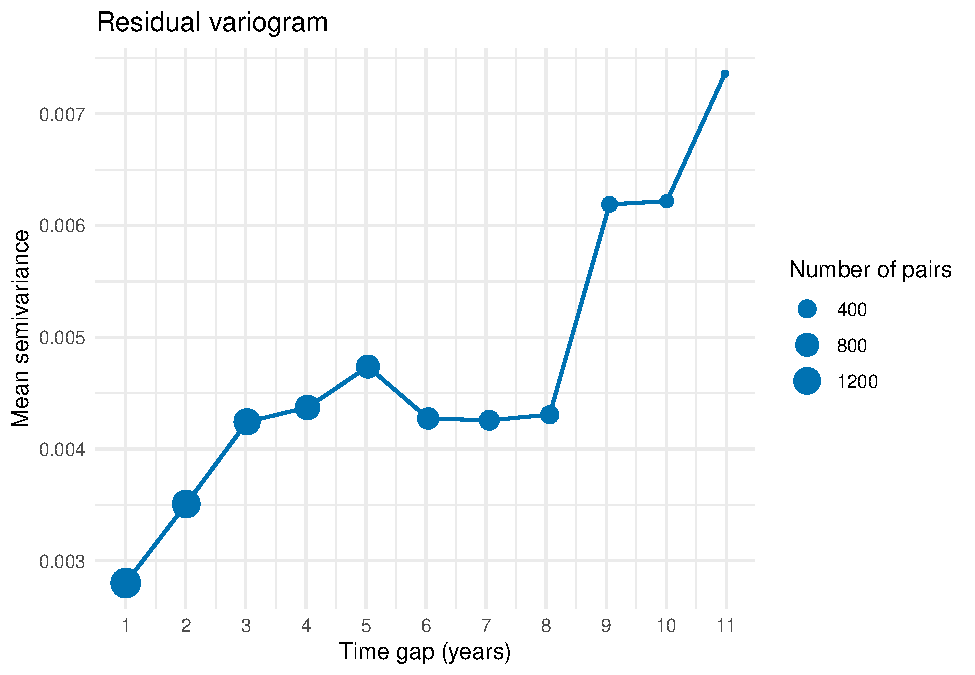
\includegraphics[keepaspectratio]{2026-10-05_p8157_hw-01_knit-to-pdf_files/figure-latex/unnamed-chunk-16-1.pdf}}

The residual variogram generally increases with the time gap, suggesting
that measurements closer in time are more strongly correlated. I will
therefore explore a correlation structure that depends on the time gap.
The estimates at long gaps are based on fewer pairs and should be
interpreted cautiously.

\begin{Shaded}
\begin{Highlighting}[]
\NormalTok{fig6\_topeka\_boxplot\_residual\_age }\OtherTok{\textless{}{-}} 
\NormalTok{  df\_topeka }\SpecialCharTok{|\textgreater{}}
  \FunctionTok{mutate}\NormalTok{(}\AttributeTok{age\_group =} \FunctionTok{floor}\NormalTok{(age)) }\SpecialCharTok{|\textgreater{}}
  \FunctionTok{ggplot}\NormalTok{(}\FunctionTok{aes}\NormalTok{(}\AttributeTok{x =} \FunctionTok{factor}\NormalTok{(age\_group), }\AttributeTok{y =}\NormalTok{ residual\_mean)) }\SpecialCharTok{+}
  \FunctionTok{geom\_hline}\NormalTok{(}\AttributeTok{yintercept =} \DecValTok{0}\NormalTok{, }\AttributeTok{linetype =} \StringTok{"dashed"}\NormalTok{, }\AttributeTok{color =} \StringTok{"grey50"}\NormalTok{) }\SpecialCharTok{+}
  \FunctionTok{geom\_boxplot}\NormalTok{(}\AttributeTok{outlier.alpha =} \FloatTok{0.4}\NormalTok{) }\SpecialCharTok{+}
  \FunctionTok{labs}\NormalTok{(}
    \AttributeTok{title =} \StringTok{"Residual spread by age"}\NormalTok{,}
    \AttributeTok{x =} \StringTok{"Age group (years)"}\NormalTok{,}
    \AttributeTok{y =} \StringTok{"Residual log(FEV1)"}
\NormalTok{  ) }\SpecialCharTok{+} \FunctionTok{theme\_minimal}\NormalTok{()}

\FunctionTok{ggsave}\NormalTok{(}\StringTok{"plots/2026{-}10{-}05\_fig06\_topeka\_residual{-}age\_boxplot.png"}\NormalTok{,}
\NormalTok{       fig6\_topeka\_boxplot\_residual\_age, }\AttributeTok{height =} \DecValTok{6}\NormalTok{, }\AttributeTok{width =} \DecValTok{9}\NormalTok{, }\AttributeTok{dpi =} \DecValTok{1200}\NormalTok{)}

\NormalTok{fig6\_topeka\_boxplot\_residual\_age}
\end{Highlighting}
\end{Shaded}

\pandocbounded{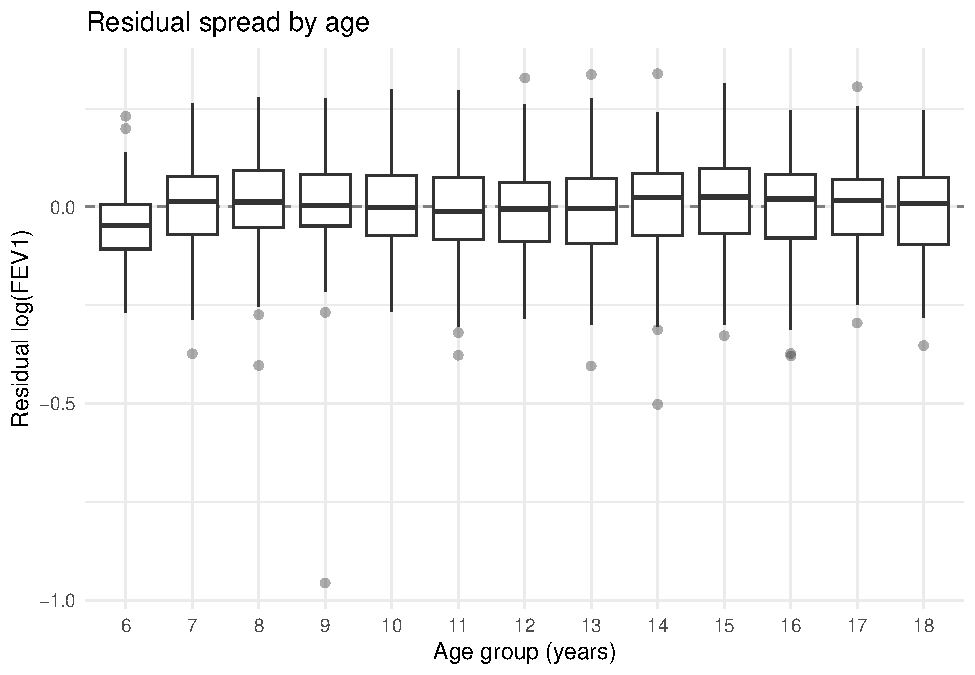
\includegraphics[keepaspectratio]{2026-10-05_p8157_hw-01_knit-to-pdf_files/figure-latex/unnamed-chunk-17-1.pdf}}

The residual spread is similar across age groups, with no clear trend in
variability. I will therefore start with a constant-variance model and
check this assumption after fitting the model.

Subject 197 has a clearly low value and only one measurement, so I
cannot compare it with her other visits.

\subsection{questions proposed}\label{questions-proposed}

\textbf{Overall trends:} How does lung function change with age on
average? Does growth slow down during the teenage years? Within girls,
is an increase in height associated with an increase in lung function?

\textbf{Individual differences:} Do girls differ in their lung function
levels and rates of growth? How strongly are repeated measurements from
the same girl correlated, and does this correlation decrease as the time
gap increases?

\subsection{single time measurement}\label{single-time-measurement}

\textbf{Overall trends:} With one measurement per girl, we could examine
how average lung function differs across ages. However, differences
between younger and older girls can't describe how the same person
changes by time. The interpretation required girls of different ages to
be comparable in other factors affecting lung function (exchangeable).
Also, baseline ages range from about 6.43 to 14 years, so these data
would not directly show whether growth slows after 15.

We could also examine if taller girls have higher lung function.
However, this would describe a between-subject association, rather than
whether a girl's lung function increases as she grows taller.

\textbf{Individual differences:} We could study differences in lung
function levels between girls of similar age and height. However, one
measurement per girl would not allow us to distinguish persistent
individual differences from temporary variation or measurement error. We
weren't able to directly estimate individual growth rates, within-girl
correlation, or how that correlation changed by time.

\section{Question 3}\label{question-3}

\subsection{table one}\label{table-one}

\begin{Shaded}
\begin{Highlighting}[]
\NormalTok{df\_eligible\_ids }\OtherTok{\textless{}{-}}\NormalTok{ macs }\SpecialCharTok{|\textgreater{}}
  \FunctionTok{group\_by}\NormalTok{(id) }\SpecialCharTok{|\textgreater{}}
  \FunctionTok{summarise}\NormalTok{(}
    \AttributeTok{has\_pre =} \FunctionTok{any}\NormalTok{(time }\SpecialCharTok{\textgreater{}=} \SpecialCharTok{{-}}\FloatTok{0.5} \SpecialCharTok{\&}\NormalTok{ time }\SpecialCharTok{\textless{}} \DecValTok{0}\NormalTok{),}
    \AttributeTok{has\_post =} \FunctionTok{any}\NormalTok{(time }\SpecialCharTok{\textgreater{}} \DecValTok{0}\NormalTok{),}
    \AttributeTok{.groups =} \StringTok{"drop"}
\NormalTok{  ) }\SpecialCharTok{|\textgreater{}}
  \FunctionTok{filter}\NormalTok{(has\_pre }\SpecialCharTok{\&}\NormalTok{ has\_post)}

\FunctionTok{nrow}\NormalTok{(df\_eligible\_ids)  }
\end{Highlighting}
\end{Shaded}

\begin{verbatim}
## [1] 266
\end{verbatim}

\begin{Shaded}
\begin{Highlighting}[]
\NormalTok{df\_macs\_baseline }\OtherTok{\textless{}{-}}\NormalTok{ macs }\SpecialCharTok{|\textgreater{}}
  \FunctionTok{semi\_join}\NormalTok{(df\_eligible\_ids, }\AttributeTok{by =} \StringTok{"id"}\NormalTok{) }\SpecialCharTok{|\textgreater{}}
  \FunctionTok{filter}\NormalTok{(time }\SpecialCharTok{\textgreater{}=} \SpecialCharTok{{-}}\FloatTok{0.5} \SpecialCharTok{\&}\NormalTok{ time }\SpecialCharTok{\textless{}} \DecValTok{0}\NormalTok{) }\SpecialCharTok{|\textgreater{}}
  \FunctionTok{arrange}\NormalTok{(id)}

\FunctionTok{nrow}\NormalTok{(df\_macs\_baseline)             }\CommentTok{\# 266}
\end{Highlighting}
\end{Shaded}

\begin{verbatim}
## [1] 266
\end{verbatim}

\begin{Shaded}
\begin{Highlighting}[]
\FunctionTok{n\_distinct}\NormalTok{(df\_macs\_baseline}\SpecialCharTok{$}\NormalTok{id)    }\CommentTok{\# 266}
\end{Highlighting}
\end{Shaded}

\begin{verbatim}
## [1] 266
\end{verbatim}

\begin{Shaded}
\begin{Highlighting}[]
\NormalTok{continuous\_row }\OtherTok{\textless{}{-}} \ControlFlowTok{function}\NormalTok{(label, x) \{}
\NormalTok{  missing\_n }\OtherTok{\textless{}{-}} \FunctionTok{sum}\NormalTok{(}\FunctionTok{is.na}\NormalTok{(x))}
\NormalTok{  x }\OtherTok{\textless{}{-}}\NormalTok{ x[}\SpecialCharTok{!}\FunctionTok{is.na}\NormalTok{(x)]}

  \FunctionTok{tibble}\NormalTok{(}
    \AttributeTok{Characteristic =}\NormalTok{ label,}
    \StringTok{\textasciigrave{}}\AttributeTok{Mean (SD) or n (\%)}\StringTok{\textasciigrave{}} \OtherTok{=}
      \FunctionTok{sprintf}\NormalTok{(}\StringTok{"\%.2f (\%.2f)"}\NormalTok{, }\FunctionTok{mean}\NormalTok{(x), }\FunctionTok{sd}\NormalTok{(x)),}
    \StringTok{\textasciigrave{}}\AttributeTok{Median [Q1, Q3]}\StringTok{\textasciigrave{}} \OtherTok{=}
      \FunctionTok{sprintf}\NormalTok{(}
        \StringTok{"\%.2f [\%.2f, \%.2f]"}\NormalTok{,}
        \FunctionTok{median}\NormalTok{(x),}
        \FunctionTok{quantile}\NormalTok{(x, }\FloatTok{0.25}\NormalTok{),}
        \FunctionTok{quantile}\NormalTok{(x, }\FloatTok{0.75}\NormalTok{)}
\NormalTok{      ),}
    \AttributeTok{Missing =} \FunctionTok{as.character}\NormalTok{(missing\_n)}
\NormalTok{  )}
\NormalTok{\}}
\end{Highlighting}
\end{Shaded}

\begin{Shaded}
\begin{Highlighting}[]
\NormalTok{categorical\_rows }\OtherTok{\textless{}{-}} \ControlFlowTok{function}\NormalTok{(label, x) \{}
\NormalTok{  missing\_n }\OtherTok{\textless{}{-}} \FunctionTok{sum}\NormalTok{(}\FunctionTok{is.na}\NormalTok{(x))}
\NormalTok{  observed }\OtherTok{\textless{}{-}}\NormalTok{ x[}\SpecialCharTok{!}\FunctionTok{is.na}\NormalTok{(x)]}
\NormalTok{  counts }\OtherTok{\textless{}{-}} \FunctionTok{table}\NormalTok{(observed)}

  \FunctionTok{bind\_rows}\NormalTok{(}
    \FunctionTok{tibble}\NormalTok{(}
      \AttributeTok{Characteristic =}\NormalTok{ label,}
      \StringTok{\textasciigrave{}}\AttributeTok{Mean (SD) or n (\%)}\StringTok{\textasciigrave{}} \OtherTok{=} \StringTok{""}\NormalTok{,}
      \StringTok{\textasciigrave{}}\AttributeTok{Median [Q1, Q3]}\StringTok{\textasciigrave{}} \OtherTok{=} \StringTok{""}\NormalTok{,}
      \AttributeTok{Missing =} \FunctionTok{as.character}\NormalTok{(missing\_n)}
\NormalTok{    ),}
    \FunctionTok{tibble}\NormalTok{(}
      \AttributeTok{Characteristic =} \FunctionTok{paste0}\NormalTok{(}\StringTok{"  Code "}\NormalTok{, }\FunctionTok{names}\NormalTok{(counts)),}
      \StringTok{\textasciigrave{}}\AttributeTok{Mean (SD) or n (\%)}\StringTok{\textasciigrave{}} \OtherTok{=} \FunctionTok{sprintf}\NormalTok{(}
        \StringTok{"\%d (\%.1f\%\%)"}\NormalTok{,}
        \FunctionTok{as.integer}\NormalTok{(counts),}
        \DecValTok{100} \SpecialCharTok{*} \FunctionTok{as.integer}\NormalTok{(counts) }\SpecialCharTok{/} \FunctionTok{length}\NormalTok{(observed)}
\NormalTok{      ),}
      \StringTok{\textasciigrave{}}\AttributeTok{Median [Q1, Q3]}\StringTok{\textasciigrave{}} \OtherTok{=} \StringTok{""}\NormalTok{,}
      \AttributeTok{Missing =} \StringTok{""}
\NormalTok{    )}
\NormalTok{  )}
\NormalTok{\}}
\end{Highlighting}
\end{Shaded}

\begin{Shaded}
\begin{Highlighting}[]
\NormalTok{table\_one }\OtherTok{\textless{}{-}} \FunctionTok{bind\_rows}\NormalTok{(}
  \FunctionTok{continuous\_row}\NormalTok{(}\StringTok{"age (original scale)"}\NormalTok{, df\_macs\_baseline}\SpecialCharTok{$}\NormalTok{age),}
  \FunctionTok{categorical\_rows}\NormalTok{(}\StringTok{"packs (original codes)"}\NormalTok{, df\_macs\_baseline}\SpecialCharTok{$}\NormalTok{packs),}
  \FunctionTok{categorical\_rows}\NormalTok{(}\StringTok{"drug (original codes)"}\NormalTok{, df\_macs\_baseline}\SpecialCharTok{$}\NormalTok{drug),}
  \FunctionTok{continuous\_row}\NormalTok{(}\StringTok{"partners (original scale)"}\NormalTok{, df\_macs\_baseline}\SpecialCharTok{$}\NormalTok{partners),}
  \FunctionTok{continuous\_row}\NormalTok{(}\StringTok{"CESD score"}\NormalTok{, df\_macs\_baseline}\SpecialCharTok{$}\NormalTok{cesd),}
  \FunctionTok{continuous\_row}\NormalTok{(}\StringTok{"Baseline CD4+ count"}\NormalTok{, df\_macs\_baseline}\SpecialCharTok{$}\NormalTok{cd4)}
\NormalTok{)}


\FunctionTok{kable}\NormalTok{(}
\NormalTok{  table\_one,}
  \AttributeTok{caption =} \StringTok{"Table 1. Baseline characteristics of the MACS sample (N = 266)"}\NormalTok{,}
  \AttributeTok{align =} \FunctionTok{c}\NormalTok{(}\StringTok{"l"}\NormalTok{, }\StringTok{"r"}\NormalTok{, }\StringTok{"r"}\NormalTok{, }\StringTok{"r"}\NormalTok{),}
  \AttributeTok{row.names =} \ConstantTok{FALSE}
\NormalTok{)}
\end{Highlighting}
\end{Shaded}

\begin{longtable}[]{@{}
  >{\raggedright\arraybackslash}p{(\linewidth - 6\tabcolsep) * \real{0.3333}}
  >{\raggedleft\arraybackslash}p{(\linewidth - 6\tabcolsep) * \real{0.2436}}
  >{\raggedleft\arraybackslash}p{(\linewidth - 6\tabcolsep) * \real{0.3205}}
  >{\raggedleft\arraybackslash}p{(\linewidth - 6\tabcolsep) * \real{0.1026}}@{}}
\caption{Table 1. Baseline characteristics of the MACS sample (N =
266)}\tabularnewline
\toprule\noalign{}
\begin{minipage}[b]{\linewidth}\raggedright
Characteristic
\end{minipage} & \begin{minipage}[b]{\linewidth}\raggedleft
Mean (SD) or n (\%)
\end{minipage} & \begin{minipage}[b]{\linewidth}\raggedleft
Median {[}Q1, Q3{]}
\end{minipage} & \begin{minipage}[b]{\linewidth}\raggedleft
Missing
\end{minipage} \\
\midrule\noalign{}
\endfirsthead
\toprule\noalign{}
\begin{minipage}[b]{\linewidth}\raggedright
Characteristic
\end{minipage} & \begin{minipage}[b]{\linewidth}\raggedleft
Mean (SD) or n (\%)
\end{minipage} & \begin{minipage}[b]{\linewidth}\raggedleft
Median {[}Q1, Q3{]}
\end{minipage} & \begin{minipage}[b]{\linewidth}\raggedleft
Missing
\end{minipage} \\
\midrule\noalign{}
\endhead
\bottomrule\noalign{}
\endlastfoot
age (original scale) & 2.34 (7.44) & 1.27 {[}-2.94, 6.33{]} & 0 \\
packs (original codes) & & & 0 \\
Code 0 & 159 (59.8\%) & & \\
Code 1 & 11 (4.1\%) & & \\
Code 2 & 16 (6.0\%) & & \\
Code 3 & 55 (20.7\%) & & \\
Code 4 & 25 (9.4\%) & & \\
drug (original codes) & & & 0 \\
Code 0 & 48 (18.0\%) & & \\
Code 1 & 218 (82.0\%) & & \\
partners (original scale) & 6.72 (3.48) & 8.00 {[}3.00, 10.00{]} & 0 \\
CESD score & 10.02 (10.04) & 7.00 {[}2.25, 14.00{]} & 0 \\
Baseline CD4+ count & 998.88 (422.43) & 932.50 {[}696.25, 1220.75{]} &
0 \\
\end{longtable}

Baseline was defined as the pre-seroconversion measurement within six
months of seroconversion. Percentages use non-missing observations as
the denominator. Variables with unconfirmed definitions are presented on
their original scales or using their original codes.

\subsection{two-stage least squares
analysis}\label{two-stage-least-squares-analysis}

\subsubsection{stage one}\label{stage-one}

\begin{Shaded}
\begin{Highlighting}[]
\NormalTok{baseline\_records }\OtherTok{\textless{}{-}}\NormalTok{ df\_macs\_baseline }\SpecialCharTok{|\textgreater{}}
  \FunctionTok{mutate}\NormalTok{(}
    \AttributeTok{time\_original =}\NormalTok{ time,}
    \AttributeTok{time =} \DecValTok{0}
\NormalTok{  )}

\NormalTok{post\_records }\OtherTok{\textless{}{-}}\NormalTok{ macs }\SpecialCharTok{|\textgreater{}}
  \FunctionTok{semi\_join}\NormalTok{(df\_eligible\_ids, }\AttributeTok{by =} \StringTok{"id"}\NormalTok{) }\SpecialCharTok{|\textgreater{}}
  \FunctionTok{filter}\NormalTok{(time }\SpecialCharTok{\textgreater{}} \DecValTok{0}\NormalTok{) }\SpecialCharTok{|\textgreater{}}
  \FunctionTok{mutate}\NormalTok{(}\AttributeTok{time\_original =}\NormalTok{ time)}


\NormalTok{df\_macs\_analysis }\OtherTok{\textless{}{-}} \FunctionTok{bind\_rows}\NormalTok{(}
\NormalTok{  baseline\_records,}
\NormalTok{  post\_records}
\NormalTok{) }\SpecialCharTok{|\textgreater{}}
  \FunctionTok{arrange}\NormalTok{(id, time)}
\end{Highlighting}
\end{Shaded}

\begin{Shaded}
\begin{Highlighting}[]
\NormalTok{stage1\_models }\OtherTok{\textless{}{-}}\NormalTok{ df\_macs\_analysis }\SpecialCharTok{|\textgreater{}}
  \FunctionTok{group\_by}\NormalTok{(id) }\SpecialCharTok{|\textgreater{}}
  \FunctionTok{nest}\NormalTok{() }\SpecialCharTok{|\textgreater{}}
  \FunctionTok{ungroup}\NormalTok{() }\SpecialCharTok{|\textgreater{}}
  \FunctionTok{mutate}\NormalTok{(}
    \AttributeTok{model =} \FunctionTok{map}\NormalTok{(data, }\SpecialCharTok{\textasciitilde{}} \FunctionTok{lm}\NormalTok{(cd4 }\SpecialCharTok{\textasciitilde{}}\NormalTok{ time, }\AttributeTok{data =}\NormalTok{ .x))}
\NormalTok{  )}
\end{Highlighting}
\end{Shaded}

\begin{Shaded}
\begin{Highlighting}[]
\NormalTok{stage1\_results }\OtherTok{\textless{}{-}}\NormalTok{ stage1\_models }\SpecialCharTok{|\textgreater{}}
  \FunctionTok{transmute}\NormalTok{(}
\NormalTok{    id,}
    \AttributeTok{n\_measurements =} \FunctionTok{map\_int}\NormalTok{(model, nobs),}
    \AttributeTok{followup\_years =} \FunctionTok{map\_dbl}\NormalTok{(data, }\SpecialCharTok{\textasciitilde{}} \FunctionTok{max}\NormalTok{(.x}\SpecialCharTok{$}\NormalTok{time)),}
    \AttributeTok{intercept =} \FunctionTok{map\_dbl}\NormalTok{(model, }\SpecialCharTok{\textasciitilde{}} \FunctionTok{unname}\NormalTok{(}\FunctionTok{coef}\NormalTok{(.x)[}\DecValTok{1}\NormalTok{])),}
    \AttributeTok{slope =} \FunctionTok{map\_dbl}\NormalTok{(model, }\SpecialCharTok{\textasciitilde{}} \FunctionTok{unname}\NormalTok{(}\FunctionTok{coef}\NormalTok{(.x)[}\DecValTok{2}\NormalTok{])),}
    \AttributeTok{slope\_se =} \FunctionTok{map\_dbl}\NormalTok{(}
\NormalTok{      model,}
      \ControlFlowTok{function}\NormalTok{(m) \{}
        \ControlFlowTok{if}\NormalTok{ (}\FunctionTok{df.residual}\NormalTok{(m) }\SpecialCharTok{\textless{}=} \DecValTok{0}\NormalTok{) }\FunctionTok{return}\NormalTok{(}\ConstantTok{NA\_real\_}\NormalTok{)}
        \FunctionTok{unname}\NormalTok{(}\FunctionTok{sqrt}\NormalTok{(}\FunctionTok{diag}\NormalTok{(}\FunctionTok{vcov}\NormalTok{(m)))[}\StringTok{"time"}\NormalTok{])}
\NormalTok{      \}}
\NormalTok{    )}
\NormalTok{  )}

\FunctionTok{head}\NormalTok{(stage1\_results)}
\end{Highlighting}
\end{Shaded}

\begin{verbatim}
## # A tibble: 6 x 6
##      id n_measurements followup_years intercept   slope slope_se
##   <int>          <int>          <dbl>     <dbl>   <dbl>    <dbl>
## 1 10002              2          0.244      893   -969.      NA  
## 2 10005              4          1.26       598.  -251.     232. 
## 3 10029              6          2.42       830.   -45.7     23.7
## 4 10039              2          0.260     1454  -2753.      NA  
## 5 10048              8          3.14       820.  -207.      64.6
## 6 10079              3          0.709      564.  -469.     352.
\end{verbatim}

\begin{Shaded}
\begin{Highlighting}[]
\NormalTok{stage1\_lines }\OtherTok{\textless{}{-}}\NormalTok{ stage1\_models }\SpecialCharTok{|\textgreater{}}
  \FunctionTok{transmute}\NormalTok{(}
\NormalTok{    id,}
    \AttributeTok{fitted\_data =} \FunctionTok{map2}\NormalTok{(}
\NormalTok{      data, model,}
      \ControlFlowTok{function}\NormalTok{(d, m) \{}
\NormalTok{        new\_data }\OtherTok{\textless{}{-}} \FunctionTok{tibble}\NormalTok{(}
          \AttributeTok{time =} \FunctionTok{seq}\NormalTok{(}\DecValTok{0}\NormalTok{, }\FunctionTok{max}\NormalTok{(d}\SpecialCharTok{$}\NormalTok{time), }\AttributeTok{length.out =} \DecValTok{50}\NormalTok{)}
\NormalTok{        )}
\NormalTok{        new\_data }\SpecialCharTok{|\textgreater{}}
          \FunctionTok{mutate}\NormalTok{(}\AttributeTok{cd4\_fitted =} \FunctionTok{as.numeric}\NormalTok{(}\FunctionTok{predict}\NormalTok{(m, new\_data)))}
\NormalTok{      \}}
\NormalTok{    )}
\NormalTok{  ) }\SpecialCharTok{|\textgreater{}}
  \FunctionTok{unnest}\NormalTok{(fitted\_data)}
\end{Highlighting}
\end{Shaded}

\begin{Shaded}
\begin{Highlighting}[]
\NormalTok{fig7\_cd4\_linear\_by\_subject }\OtherTok{\textless{}{-}} 
  \FunctionTok{ggplot}\NormalTok{() }\SpecialCharTok{+}
  \FunctionTok{geom\_line}\NormalTok{(}
    \AttributeTok{data =}\NormalTok{ df\_macs\_analysis,}
    \FunctionTok{aes}\NormalTok{(time, cd4, }\AttributeTok{group =}\NormalTok{ id),}
    \AttributeTok{color =} \StringTok{"grey60"}\NormalTok{, }\AttributeTok{alpha =} \FloatTok{0.15}
\NormalTok{  ) }\SpecialCharTok{+}
  \FunctionTok{geom\_line}\NormalTok{(}
    \AttributeTok{data =}\NormalTok{ stage1\_lines,}
    \FunctionTok{aes}\NormalTok{(time, cd4\_fitted, }\AttributeTok{group =}\NormalTok{ id),}
    \AttributeTok{color =} \StringTok{"\#0072B2"}\NormalTok{, }\AttributeTok{alpha =} \FloatTok{0.25}
\NormalTok{  ) }\SpecialCharTok{+}
  \FunctionTok{labs}\NormalTok{(}
    \AttributeTok{title =} \StringTok{"Individual linear fits for CD4+ count"}\NormalTok{,}
    \AttributeTok{x =} \StringTok{"Time since seroconversion (years; baseline treated as 0)"}\NormalTok{,}
    \AttributeTok{y =} \StringTok{"CD4+ count"}
\NormalTok{  ) }\SpecialCharTok{+}
  \FunctionTok{theme\_minimal}\NormalTok{()}

\FunctionTok{ggsave}\NormalTok{(}\StringTok{"plots/2026{-}10{-}06\_fig07\_cd4\_linear{-}by{-}subject.png"}\NormalTok{, }
\NormalTok{       fig7\_cd4\_linear\_by\_subject, }\AttributeTok{height =} \DecValTok{6}\NormalTok{, }\AttributeTok{width =} \DecValTok{9}\NormalTok{, }\AttributeTok{dpi =} \DecValTok{900}\NormalTok{)}

\NormalTok{fig7\_cd4\_linear\_by\_subject}
\end{Highlighting}
\end{Shaded}

\pandocbounded{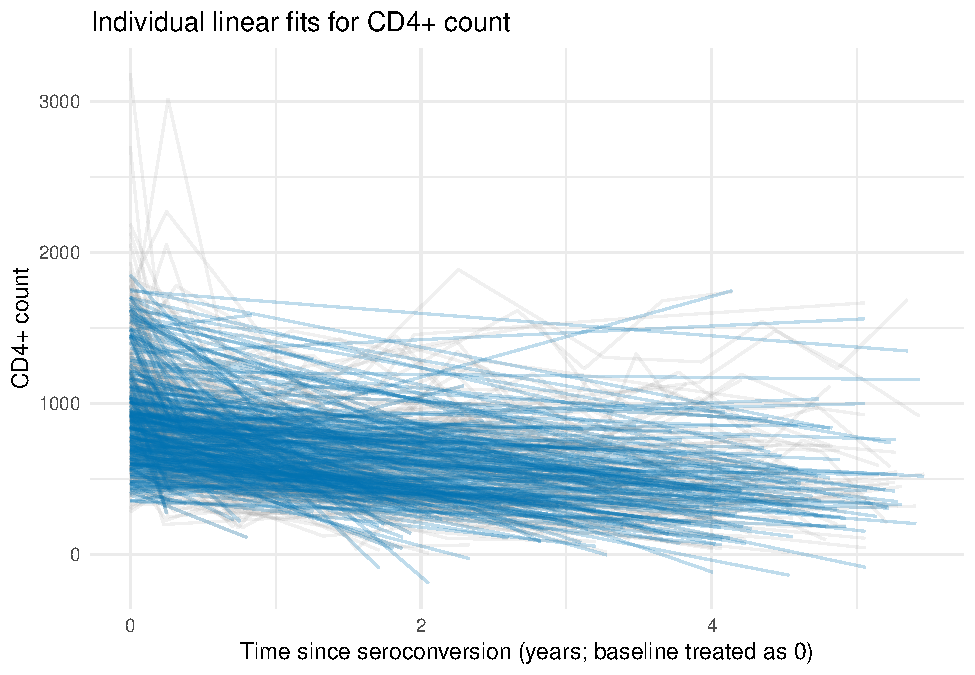
\includegraphics[keepaspectratio]{2026-10-05_p8157_hw-01_knit-to-pdf_files/figure-latex/unnamed-chunk-27-1.pdf}}

\subsubsection{stage two}\label{stage-two}

\begin{Shaded}
\begin{Highlighting}[]
\NormalTok{stage1\_results }\SpecialCharTok{|\textgreater{}}
  \FunctionTok{summarise}\NormalTok{(}
    \AttributeTok{n\_subjects =} \FunctionTok{n}\NormalTok{(),}
    \AttributeTok{mean\_slope =} \FunctionTok{mean}\NormalTok{(slope),}
    \AttributeTok{median\_slope =} \FunctionTok{median}\NormalTok{(slope),}
    \AttributeTok{q1\_slope =} \FunctionTok{quantile}\NormalTok{(slope, }\FloatTok{0.25}\NormalTok{),}
    \AttributeTok{q3\_slope =} \FunctionTok{quantile}\NormalTok{(slope, }\FloatTok{0.75}\NormalTok{),}
    \AttributeTok{percent\_negative =} \DecValTok{100} \SpecialCharTok{*} \FunctionTok{mean}\NormalTok{(slope }\SpecialCharTok{\textless{}} \DecValTok{0}\NormalTok{),}
    \AttributeTok{n\_two\_measurements =} \FunctionTok{sum}\NormalTok{(n\_measurements }\SpecialCharTok{==} \DecValTok{2}\NormalTok{)}
\NormalTok{  )}
\end{Highlighting}
\end{Shaded}

\begin{verbatim}
## # A tibble: 1 x 7
##   n_subjects mean_slope median_slope q1_slope q3_slope percent_negative
##        <int>      <dbl>        <dbl>    <dbl>    <dbl>            <dbl>
## 1        266      -293.        -142.    -284.    -67.5             92.5
## # i 1 more variable: n_two_measurements <int>
\end{verbatim}

\begin{Shaded}
\begin{Highlighting}[]
\NormalTok{stage2\_data }\OtherTok{\textless{}{-}}\NormalTok{ stage1\_results }\SpecialCharTok{|\textgreater{}}
  \FunctionTok{left\_join}\NormalTok{(}
\NormalTok{    df\_macs\_baseline }\SpecialCharTok{|\textgreater{}}
      \FunctionTok{select}\NormalTok{(id, age, packs, drug, partners, cesd),}
    \AttributeTok{by =} \StringTok{"id"}
\NormalTok{  ) }\SpecialCharTok{|\textgreater{}}
  \FunctionTok{mutate}\NormalTok{(}
    \AttributeTok{packs =} \FunctionTok{factor}\NormalTok{(packs),}
    \AttributeTok{drug =} \FunctionTok{factor}\NormalTok{(drug)}
\NormalTok{  )}

\NormalTok{stage2\_intercept }\OtherTok{\textless{}{-}} \FunctionTok{lm}\NormalTok{(}
\NormalTok{  intercept }\SpecialCharTok{\textasciitilde{}}\NormalTok{ age }\SpecialCharTok{+}\NormalTok{ packs }\SpecialCharTok{+}\NormalTok{ drug }\SpecialCharTok{+}\NormalTok{ partners }\SpecialCharTok{+}\NormalTok{ cesd,}
  \AttributeTok{data =}\NormalTok{ stage2\_data}
\NormalTok{)}

\NormalTok{stage2\_slope }\OtherTok{\textless{}{-}} \FunctionTok{lm}\NormalTok{(}
\NormalTok{  slope }\SpecialCharTok{\textasciitilde{}}\NormalTok{ age }\SpecialCharTok{+}\NormalTok{ packs }\SpecialCharTok{+}\NormalTok{ drug }\SpecialCharTok{+}\NormalTok{ partners }\SpecialCharTok{+}\NormalTok{ cesd,}
  \AttributeTok{data =}\NormalTok{ stage2\_data}
\NormalTok{)}

\FunctionTok{summary}\NormalTok{(stage2\_intercept)}
\end{Highlighting}
\end{Shaded}

\begin{verbatim}
## 
## Call:
## lm(formula = intercept ~ age + packs + drug + partners + cesd, 
##     data = stage2_data)
## 
## Residuals:
##     Min      1Q  Median      3Q     Max 
## -817.66 -210.88  -47.96  149.72  972.40 
## 
## Coefficients:
##             Estimate Std. Error t value Pr(>|t|)    
## (Intercept)  798.096     57.956  13.771  < 2e-16 ***
## age            2.654      2.635   1.007   0.3149    
## packs1       -76.160     94.054  -0.810   0.4188    
## packs2       152.466     80.219   1.901   0.0585 .  
## packs3       319.687     47.503   6.730  1.1e-10 ***
## packs4       143.637     66.454   2.161   0.0316 *  
## drug1        113.708     49.923   2.278   0.0236 *  
## partners      -8.375      5.436  -1.541   0.1246    
## cesd          -2.101      1.882  -1.116   0.2653    
## ---
## Signif. codes:  0 '***' 0.001 '**' 0.01 '*' 0.05 '.' 0.1 ' ' 1
## 
## Residual standard error: 300.4 on 257 degrees of freedom
## Multiple R-squared:  0.198,  Adjusted R-squared:  0.173 
## F-statistic: 7.931 on 8 and 257 DF,  p-value: 1.538e-09
\end{verbatim}

\begin{Shaded}
\begin{Highlighting}[]
\FunctionTok{summary}\NormalTok{(stage2\_slope)}
\end{Highlighting}
\end{Shaded}

\begin{verbatim}
## 
## Call:
## lm(formula = slope ~ age + packs + drug + partners + cesd, data = stage2_data)
## 
## Residuals:
##     Min      1Q  Median      3Q     Max 
## -3326.0   -26.2   134.6   235.2   562.8 
## 
## Coefficients:
##             Estimate Std. Error t value Pr(>|t|)   
## (Intercept) -272.297     97.139  -2.803  0.00545 **
## age           -3.094      4.417  -0.700  0.48428   
## packs1       221.629    157.644   1.406  0.16097   
## packs2      -120.886    134.454  -0.899  0.36945   
## packs3      -117.525     79.620  -1.476  0.14115   
## packs4       118.338    111.382   1.062  0.28903   
## drug1        -62.248     83.676  -0.744  0.45760   
## partners       2.671      9.111   0.293  0.76962   
## cesd           3.041      3.154   0.964  0.33580   
## ---
## Signif. codes:  0 '***' 0.001 '**' 0.01 '*' 0.05 '.' 0.1 ' ' 1
## 
## Residual standard error: 503.4 on 257 degrees of freedom
## Multiple R-squared:  0.03472,    Adjusted R-squared:  0.004677 
## F-statistic: 1.156 on 8 and 257 DF,  p-value: 0.3267
\end{verbatim}

\begin{Shaded}
\begin{Highlighting}[]
\NormalTok{stage1\_results }\SpecialCharTok{|\textgreater{}}
  \FunctionTok{arrange}\NormalTok{(slope) }\SpecialCharTok{|\textgreater{}}
  \FunctionTok{select}\NormalTok{(id, n\_measurements, followup\_years, slope, slope\_se) }\SpecialCharTok{|\textgreater{}}
  \FunctionTok{slice\_head}\NormalTok{(}\AttributeTok{n =} \DecValTok{10}\NormalTok{)}
\end{Highlighting}
\end{Shaded}

\begin{verbatim}
## # A tibble: 10 x 5
##       id n_measurements followup_years  slope slope_se
##    <int>          <int>          <dbl>  <dbl>    <dbl>
##  1 30132              2          0.249 -3580.       NA
##  2 40374              2          0.131 -2785.       NA
##  3 10039              2          0.260 -2753.       NA
##  4 30654              2          0.241 -2557.       NA
##  5 10372              2          0.375 -2213.       NA
##  6 20837              2          0.230 -2152.       NA
##  7 10878              2          0.241 -2138.       NA
##  8 41659              2          0.356 -2009.       NA
##  9 30183              2          0.268 -1979.       NA
## 10 40438              2          0.268 -1975.       NA
\end{verbatim}

\begin{Shaded}
\begin{Highlighting}[]
\NormalTok{stage2\_data }\SpecialCharTok{|\textgreater{}}
  \FunctionTok{mutate}\NormalTok{(}\AttributeTok{cooks\_distance =} \FunctionTok{cooks.distance}\NormalTok{(stage2\_slope)) }\SpecialCharTok{|\textgreater{}}
  \FunctionTok{arrange}\NormalTok{(}\FunctionTok{desc}\NormalTok{(cooks\_distance)) }\SpecialCharTok{|\textgreater{}}
  \FunctionTok{select}\NormalTok{(id, n\_measurements, followup\_years,}
\NormalTok{         slope, cooks\_distance) }\SpecialCharTok{|\textgreater{}}
  \FunctionTok{slice\_head}\NormalTok{(}\AttributeTok{n =} \DecValTok{10}\NormalTok{)}
\end{Highlighting}
\end{Shaded}

\begin{verbatim}
## # A tibble: 10 x 5
##       id n_measurements followup_years  slope cooks_distance
##    <int>          <int>          <dbl>  <dbl>          <dbl>
##  1 30654              2          0.241 -2557.         0.186 
##  2 10039              2          0.260 -2753.         0.0912
##  3 30132              2          0.249 -3580.         0.0653
##  4 30049              2          0.249 -1858.         0.0554
##  5 10372              2          0.375 -2213.         0.0482
##  6 40438              2          0.268 -1975.         0.0443
##  7 40374              2          0.131 -2785.         0.0363
##  8 41659              2          0.356 -2009.         0.0339
##  9 20837              2          0.230 -2152.         0.0304
## 10 10878              2          0.241 -2138.         0.0186
\end{verbatim}

\begin{Shaded}
\begin{Highlighting}[]
\NormalTok{stage2\_data\_3plus }\OtherTok{\textless{}{-}}\NormalTok{ stage2\_data }\SpecialCharTok{|\textgreater{}}
  \FunctionTok{filter}\NormalTok{(n\_measurements }\SpecialCharTok{\textgreater{}=} \DecValTok{3}\NormalTok{)}

\NormalTok{stage2\_intercept\_3plus }\OtherTok{\textless{}{-}} \FunctionTok{lm}\NormalTok{(}
\NormalTok{  intercept }\SpecialCharTok{\textasciitilde{}}\NormalTok{ age }\SpecialCharTok{+}\NormalTok{ packs }\SpecialCharTok{+}\NormalTok{ drug }\SpecialCharTok{+}\NormalTok{ partners }\SpecialCharTok{+}\NormalTok{ cesd,}
  \AttributeTok{data =}\NormalTok{ stage2\_data\_3plus}
\NormalTok{)}

\NormalTok{stage2\_slope\_3plus }\OtherTok{\textless{}{-}} \FunctionTok{lm}\NormalTok{(}
\NormalTok{  slope }\SpecialCharTok{\textasciitilde{}}\NormalTok{ age }\SpecialCharTok{+}\NormalTok{ packs }\SpecialCharTok{+}\NormalTok{ drug }\SpecialCharTok{+}\NormalTok{ partners }\SpecialCharTok{+}\NormalTok{ cesd,}
  \AttributeTok{data =}\NormalTok{ stage2\_data\_3plus}
\NormalTok{)}

\FunctionTok{summary}\NormalTok{(stage2\_intercept\_3plus)}
\end{Highlighting}
\end{Shaded}

\begin{verbatim}
## 
## Call:
## lm(formula = intercept ~ age + packs + drug + partners + cesd, 
##     data = stage2_data_3plus)
## 
## Residuals:
##     Min      1Q  Median      3Q     Max 
## -793.21 -198.00  -35.09  134.39  993.93 
## 
## Coefficients:
##             Estimate Std. Error t value Pr(>|t|)    
## (Intercept) 781.4704    60.9538  12.821  < 2e-16 ***
## age           0.0323     2.6798   0.012   0.9904    
## packs1      -49.4582    94.7644  -0.522   0.6023    
## packs2      128.6607    81.9129   1.571   0.1177    
## packs3      332.7885    49.3571   6.742 1.33e-10 ***
## packs4      168.4524    67.6924   2.488   0.0136 *  
## drug1        77.6638    51.5931   1.505   0.1337    
## partners     -3.6330     5.6878  -0.639   0.5237    
## cesd         -2.4842     1.9140  -1.298   0.1957    
## ---
## Signif. codes:  0 '***' 0.001 '**' 0.01 '*' 0.05 '.' 0.1 ' ' 1
## 
## Residual standard error: 288.1 on 222 degrees of freedom
## Multiple R-squared:  0.2031, Adjusted R-squared:  0.1744 
## F-statistic: 7.072 on 8 and 222 DF,  p-value: 2.549e-08
\end{verbatim}

\begin{Shaded}
\begin{Highlighting}[]
\FunctionTok{summary}\NormalTok{(stage2\_slope\_3plus)}
\end{Highlighting}
\end{Shaded}

\begin{verbatim}
## 
## Call:
## lm(formula = slope ~ age + packs + drug + partners + cesd, data = stage2_data_3plus)
## 
## Residuals:
##      Min       1Q   Median       3Q      Max 
## -1112.49   -67.96    36.22   106.15   444.86 
## 
## Coefficients:
##              Estimate Std. Error t value Pr(>|t|)    
## (Intercept) -128.1312    42.6978  -3.001   0.0030 ** 
## age            0.9414     1.8772   0.502   0.6165    
## packs1        81.2694    66.3820   1.224   0.2221    
## packs2       -70.0309    57.3796  -1.220   0.2236    
## packs3      -143.8673    34.5744  -4.161 4.53e-05 ***
## packs4       -31.6317    47.4182  -0.667   0.5054    
## drug1        -11.1696    36.1407  -0.309   0.7576    
## partners      -5.7808     3.9842  -1.451   0.1482    
## cesd           3.1115     1.3407   2.321   0.0212 *  
## ---
## Signif. codes:  0 '***' 0.001 '**' 0.01 '*' 0.05 '.' 0.1 ' ' 1
## 
## Residual standard error: 201.8 on 222 degrees of freedom
## Multiple R-squared:  0.1162, Adjusted R-squared:  0.0844 
## F-statistic:  3.65 on 8 and 222 DF,  p-value: 0.0005141
\end{verbatim}

\begin{Shaded}
\begin{Highlighting}[]
\NormalTok{stage2\_table }\OtherTok{\textless{}{-}} \FunctionTok{bind\_rows}\NormalTok{(}
  \FunctionTok{tidy}\NormalTok{(stage2\_intercept, }\AttributeTok{conf.int =} \ConstantTok{TRUE}\NormalTok{) }\SpecialCharTok{|\textgreater{}}
    \FunctionTok{mutate}\NormalTok{(}\AttributeTok{Model =} \StringTok{"Starting CD4 level"}\NormalTok{),}
  \FunctionTok{tidy}\NormalTok{(stage2\_slope, }\AttributeTok{conf.int =} \ConstantTok{TRUE}\NormalTok{) }\SpecialCharTok{|\textgreater{}}
    \FunctionTok{mutate}\NormalTok{(}\AttributeTok{Model =} \StringTok{"Annual CD4 change"}\NormalTok{)}
\NormalTok{) }\SpecialCharTok{|\textgreater{}}
  \FunctionTok{select}\NormalTok{(}
\NormalTok{    Model,}
    \AttributeTok{Predictor =}\NormalTok{ term,}
    \AttributeTok{Estimate =}\NormalTok{ estimate,}
    \StringTok{\textasciigrave{}}\AttributeTok{Lower 95\% CI}\StringTok{\textasciigrave{}} \OtherTok{=}\NormalTok{ conf.low,}
    \StringTok{\textasciigrave{}}\AttributeTok{Upper 95\% CI}\StringTok{\textasciigrave{}} \OtherTok{=}\NormalTok{ conf.high,}
    \StringTok{\textasciigrave{}}\AttributeTok{p{-}value}\StringTok{\textasciigrave{}} \OtherTok{=}\NormalTok{ p.value}
\NormalTok{  )}

\FunctionTok{kable}\NormalTok{(}
\NormalTok{  stage2\_table,}
  \AttributeTok{digits =} \DecValTok{3}\NormalTok{,}
  \AttributeTok{caption =} \StringTok{"Stage{-}two regression results"}
\NormalTok{)}
\end{Highlighting}
\end{Shaded}

\begin{longtable}[]{@{}
  >{\raggedright\arraybackslash}p{(\linewidth - 10\tabcolsep) * \real{0.2568}}
  >{\raggedright\arraybackslash}p{(\linewidth - 10\tabcolsep) * \real{0.1622}}
  >{\raggedleft\arraybackslash}p{(\linewidth - 10\tabcolsep) * \real{0.1216}}
  >{\raggedleft\arraybackslash}p{(\linewidth - 10\tabcolsep) * \real{0.1757}}
  >{\raggedleft\arraybackslash}p{(\linewidth - 10\tabcolsep) * \real{0.1757}}
  >{\raggedleft\arraybackslash}p{(\linewidth - 10\tabcolsep) * \real{0.1081}}@{}}
\caption{Stage-two regression results}\tabularnewline
\toprule\noalign{}
\begin{minipage}[b]{\linewidth}\raggedright
Model
\end{minipage} & \begin{minipage}[b]{\linewidth}\raggedright
Predictor
\end{minipage} & \begin{minipage}[b]{\linewidth}\raggedleft
Estimate
\end{minipage} & \begin{minipage}[b]{\linewidth}\raggedleft
Lower 95\% CI
\end{minipage} & \begin{minipage}[b]{\linewidth}\raggedleft
Upper 95\% CI
\end{minipage} & \begin{minipage}[b]{\linewidth}\raggedleft
p-value
\end{minipage} \\
\midrule\noalign{}
\endfirsthead
\toprule\noalign{}
\begin{minipage}[b]{\linewidth}\raggedright
Model
\end{minipage} & \begin{minipage}[b]{\linewidth}\raggedright
Predictor
\end{minipage} & \begin{minipage}[b]{\linewidth}\raggedleft
Estimate
\end{minipage} & \begin{minipage}[b]{\linewidth}\raggedleft
Lower 95\% CI
\end{minipage} & \begin{minipage}[b]{\linewidth}\raggedleft
Upper 95\% CI
\end{minipage} & \begin{minipage}[b]{\linewidth}\raggedleft
p-value
\end{minipage} \\
\midrule\noalign{}
\endhead
\bottomrule\noalign{}
\endlastfoot
Starting CD4 level & (Intercept) & 798.096 & 683.967 & 912.224 &
0.000 \\
Starting CD4 level & age & 2.654 & -2.536 & 7.843 & 0.315 \\
Starting CD4 level & packs1 & -76.160 & -261.375 & 109.055 & 0.419 \\
Starting CD4 level & packs2 & 152.466 & -5.504 & 310.436 & 0.058 \\
Starting CD4 level & packs3 & 319.687 & 226.142 & 413.232 & 0.000 \\
Starting CD4 level & packs4 & 143.637 & 12.774 & 274.500 & 0.032 \\
Starting CD4 level & drug1 & 113.708 & 15.398 & 212.019 & 0.024 \\
Starting CD4 level & partners & -8.375 & -19.080 & 2.330 & 0.125 \\
Starting CD4 level & cesd & -2.101 & -5.806 & 1.604 & 0.265 \\
Annual CD4 change & (Intercept) & -272.297 & -463.587 & -81.007 &
0.005 \\
Annual CD4 change & age & -3.094 & -11.792 & 5.604 & 0.484 \\
Annual CD4 change & packs1 & 221.629 & -88.809 & 532.066 & 0.161 \\
Annual CD4 change & packs2 & -120.886 & -385.658 & 143.886 & 0.369 \\
Annual CD4 change & packs3 & -117.525 & -274.315 & 39.265 & 0.141 \\
Annual CD4 change & packs4 & 118.338 & -101.000 & 337.677 & 0.289 \\
Annual CD4 change & drug1 & -62.248 & -227.026 & 102.530 & 0.458 \\
Annual CD4 change & partners & 2.671 & -15.271 & 20.613 & 0.770 \\
Annual CD4 change & cesd & 3.041 & -3.169 & 9.251 & 0.336 \\
\end{longtable}

\begin{Shaded}
\begin{Highlighting}[]
\NormalTok{check\_ids }\OtherTok{\textless{}{-}}\NormalTok{ stage2\_data }\SpecialCharTok{|\textgreater{}}
  \FunctionTok{mutate}\NormalTok{(}\AttributeTok{cooks\_distance =} \FunctionTok{cooks.distance}\NormalTok{(stage2\_slope)) }\SpecialCharTok{|\textgreater{}}
  \FunctionTok{arrange}\NormalTok{(}\FunctionTok{desc}\NormalTok{(cooks\_distance)) }\SpecialCharTok{|\textgreater{}}
  \FunctionTok{slice\_head}\NormalTok{(}\AttributeTok{n =} \DecValTok{5}\NormalTok{) }\SpecialCharTok{|\textgreater{}}
  \FunctionTok{pull}\NormalTok{(id)}

\NormalTok{df\_macs\_analysis }\SpecialCharTok{|\textgreater{}}
  \FunctionTok{filter}\NormalTok{(id }\SpecialCharTok{\%in\%}\NormalTok{ check\_ids) }\SpecialCharTok{|\textgreater{}}
  \FunctionTok{arrange}\NormalTok{(id, time\_original) }\SpecialCharTok{|\textgreater{}}
  \FunctionTok{select}\NormalTok{(id, time\_original, time, cd4)}
\end{Highlighting}
\end{Shaded}

\begin{verbatim}
##       id time_original     time  cd4
## 1  10039     -0.260096 0.000000 1454
## 2  10039      0.260096 0.260096  738
## 3  10372     -0.375086 0.000000 1615
## 4  10372      0.375086 0.375086  785
## 5  30049     -0.249144 0.000000 1407
## 6  30049      0.249144 0.249144  944
## 7  30132     -0.249144 0.000000 1166
## 8  30132      0.249144 0.249144  274
## 9  30654     -0.240931 0.000000  932
## 10 30654      0.240931 0.240931  316
\end{verbatim}

\begin{Shaded}
\begin{Highlighting}[]
\NormalTok{comparison\_table }\OtherTok{\textless{}{-}} \FunctionTok{bind\_rows}\NormalTok{(}
  \FunctionTok{tidy}\NormalTok{(stage2\_intercept, }\AttributeTok{conf.int =} \ConstantTok{TRUE}\NormalTok{) }\SpecialCharTok{|\textgreater{}}
    \FunctionTok{mutate}\NormalTok{(}\AttributeTok{Analysis =} \StringTok{"All participants"}\NormalTok{,}
           \AttributeTok{Outcome =} \StringTok{"Starting CD4 level"}\NormalTok{),}

  \FunctionTok{tidy}\NormalTok{(stage2\_intercept\_3plus, }\AttributeTok{conf.int =} \ConstantTok{TRUE}\NormalTok{) }\SpecialCharTok{|\textgreater{}}
    \FunctionTok{mutate}\NormalTok{(}\AttributeTok{Analysis =} \StringTok{"At least 3 measurements"}\NormalTok{,}
           \AttributeTok{Outcome =} \StringTok{"Starting CD4 level"}\NormalTok{),}

  \FunctionTok{tidy}\NormalTok{(stage2\_slope, }\AttributeTok{conf.int =} \ConstantTok{TRUE}\NormalTok{) }\SpecialCharTok{|\textgreater{}}
    \FunctionTok{mutate}\NormalTok{(}\AttributeTok{Analysis =} \StringTok{"All participants"}\NormalTok{,}
           \AttributeTok{Outcome =} \StringTok{"Annual CD4 change"}\NormalTok{),}

  \FunctionTok{tidy}\NormalTok{(stage2\_slope\_3plus, }\AttributeTok{conf.int =} \ConstantTok{TRUE}\NormalTok{) }\SpecialCharTok{|\textgreater{}}
    \FunctionTok{mutate}\NormalTok{(}\AttributeTok{Analysis =} \StringTok{"At least 3 measurements"}\NormalTok{,}
           \AttributeTok{Outcome =} \StringTok{"Annual CD4 change"}\NormalTok{)}
\NormalTok{) }\SpecialCharTok{|\textgreater{}}
  \FunctionTok{filter}\NormalTok{(term }\SpecialCharTok{!=} \StringTok{"(Intercept)"}\NormalTok{) }\SpecialCharTok{|\textgreater{}}
  \FunctionTok{mutate}\NormalTok{(}
    \StringTok{\textasciigrave{}}\AttributeTok{Estimate (95\% CI)}\StringTok{\textasciigrave{}} \OtherTok{=} \FunctionTok{sprintf}\NormalTok{(}
      \StringTok{"\%.2f (\%.2f, \%.2f)"}\NormalTok{, estimate, conf.low, conf.high}
\NormalTok{    ),}
    \StringTok{\textasciigrave{}}\AttributeTok{p{-}value}\StringTok{\textasciigrave{}} \OtherTok{=} \FunctionTok{trimws}\NormalTok{(}
      \FunctionTok{format.pval}\NormalTok{(p.value, }\AttributeTok{digits =} \DecValTok{3}\NormalTok{, }\AttributeTok{eps =} \FloatTok{0.001}\NormalTok{)}
\NormalTok{    )}
\NormalTok{  ) }\SpecialCharTok{|\textgreater{}}
  \FunctionTok{select}\NormalTok{(}
\NormalTok{    Outcome, }\AttributeTok{Predictor =}\NormalTok{ term, Analysis,}
    \StringTok{\textasciigrave{}}\AttributeTok{Estimate (95\% CI)}\StringTok{\textasciigrave{}}\NormalTok{, }\StringTok{\textasciigrave{}}\AttributeTok{p{-}value}\StringTok{\textasciigrave{}}
\NormalTok{  ) }\SpecialCharTok{|\textgreater{}}
  \FunctionTok{arrange}\NormalTok{(Outcome, Predictor, Analysis)}

\FunctionTok{kable}\NormalTok{(}
\NormalTok{  comparison\_table,}
  \AttributeTok{caption =} \StringTok{"Main and sensitivity analyses"}
\NormalTok{)}
\end{Highlighting}
\end{Shaded}

\begin{longtable}[]{@{}
  >{\raggedright\arraybackslash}p{(\linewidth - 8\tabcolsep) * \real{0.2184}}
  >{\raggedright\arraybackslash}p{(\linewidth - 8\tabcolsep) * \real{0.1149}}
  >{\raggedright\arraybackslash}p{(\linewidth - 8\tabcolsep) * \real{0.2759}}
  >{\raggedright\arraybackslash}p{(\linewidth - 8\tabcolsep) * \real{0.2989}}
  >{\raggedright\arraybackslash}p{(\linewidth - 8\tabcolsep) * \real{0.0920}}@{}}
\caption{Main and sensitivity analyses}\tabularnewline
\toprule\noalign{}
\begin{minipage}[b]{\linewidth}\raggedright
Outcome
\end{minipage} & \begin{minipage}[b]{\linewidth}\raggedright
Predictor
\end{minipage} & \begin{minipage}[b]{\linewidth}\raggedright
Analysis
\end{minipage} & \begin{minipage}[b]{\linewidth}\raggedright
Estimate (95\% CI)
\end{minipage} & \begin{minipage}[b]{\linewidth}\raggedright
p-value
\end{minipage} \\
\midrule\noalign{}
\endfirsthead
\toprule\noalign{}
\begin{minipage}[b]{\linewidth}\raggedright
Outcome
\end{minipage} & \begin{minipage}[b]{\linewidth}\raggedright
Predictor
\end{minipage} & \begin{minipage}[b]{\linewidth}\raggedright
Analysis
\end{minipage} & \begin{minipage}[b]{\linewidth}\raggedright
Estimate (95\% CI)
\end{minipage} & \begin{minipage}[b]{\linewidth}\raggedright
p-value
\end{minipage} \\
\midrule\noalign{}
\endhead
\bottomrule\noalign{}
\endlastfoot
Annual CD4 change & age & All participants & -3.09 (-11.79, 5.60) &
0.4843 \\
Annual CD4 change & age & At least 3 measurements & 0.94 (-2.76, 4.64) &
0.6165 \\
Annual CD4 change & cesd & All participants & 3.04 (-3.17, 9.25) &
0.3358 \\
Annual CD4 change & cesd & At least 3 measurements & 3.11 (0.47, 5.75) &
0.0212 \\
Annual CD4 change & drug1 & All participants & -62.25 (-227.03, 102.53)
& 0.4576 \\
Annual CD4 change & drug1 & At least 3 measurements & -11.17 (-82.39,
60.05) & 0.7576 \\
Annual CD4 change & packs1 & All participants & 221.63 (-88.81, 532.07)
& 0.1610 \\
Annual CD4 change & packs1 & At least 3 measurements & 81.27 (-49.55,
212.09) & 0.2221 \\
Annual CD4 change & packs2 & All participants & -120.89 (-385.66,
143.89) & 0.3694 \\
Annual CD4 change & packs2 & At least 3 measurements & -70.03 (-183.11,
43.05) & 0.2236 \\
Annual CD4 change & packs3 & All participants & -117.53 (-274.32, 39.26)
& 0.1411 \\
Annual CD4 change & packs3 & At least 3 measurements & -143.87 (-212.00,
-75.73) & \textless0.001 \\
Annual CD4 change & packs4 & All participants & 118.34 (-101.00, 337.68)
& 0.2890 \\
Annual CD4 change & packs4 & At least 3 measurements & -31.63 (-125.08,
61.82) & 0.5054 \\
Annual CD4 change & partners & All participants & 2.67 (-15.27, 20.61) &
0.7696 \\
Annual CD4 change & partners & At least 3 measurements & -5.78 (-13.63,
2.07) & 0.1482 \\
Starting CD4 level & age & All participants & 2.65 (-2.54, 7.84) &
0.3149 \\
Starting CD4 level & age & At least 3 measurements & 0.03 (-5.25, 5.31)
& 0.9904 \\
Starting CD4 level & cesd & All participants & -2.10 (-5.81, 1.60) &
0.2653 \\
Starting CD4 level & cesd & At least 3 measurements & -2.48 (-6.26,
1.29) & 0.1957 \\
Starting CD4 level & drug1 & All participants & 113.71 (15.40, 212.02) &
0.0236 \\
Starting CD4 level & drug1 & At least 3 measurements & 77.66 (-24.01,
179.34) & 0.1337 \\
Starting CD4 level & packs1 & All participants & -76.16 (-261.38,
109.05) & 0.4188 \\
Starting CD4 level & packs1 & At least 3 measurements & -49.46 (-236.21,
137.29) & 0.6023 \\
Starting CD4 level & packs2 & All participants & 152.47 (-5.50, 310.44)
& 0.0585 \\
Starting CD4 level & packs2 & At least 3 measurements & 128.66 (-32.77,
290.09) & 0.1177 \\
Starting CD4 level & packs3 & All participants & 319.69 (226.14, 413.23)
& \textless0.001 \\
Starting CD4 level & packs3 & At least 3 measurements & 332.79 (235.52,
430.06) & \textless0.001 \\
Starting CD4 level & packs4 & All participants & 143.64 (12.77, 274.50)
& 0.0316 \\
Starting CD4 level & packs4 & At least 3 measurements & 168.45 (35.05,
301.85) & 0.0136 \\
Starting CD4 level & partners & All participants & -8.37 (-19.08, 2.33)
& 0.1246 \\
Starting CD4 level & partners & At least 3 measurements & -3.63 (-14.84,
7.58) & 0.5237 \\
\end{longtable}

I fitted a separate linear regression of CD4 count on time for each of
the 266 participants, then modeled the estimated starting CD4 levels and
annual changes using baseline covariates.

Most participants showed declining CD4 counts: 92.5\% had negative
slopes. The median slope was −141.7 per year, with an interquartile
range of −283.7 to −67.5. The mean was more negative (−293.4),
reflecting several extreme slopes.

After adjustment for the other covariates, packs codes 3 and 4 were
associated with higher estimated starting CD4 levels than code 0. Drug
code 1 was also associated with a higher starting level. None of the
baseline covariates showed a clear association with annual CD4 change in
the main analysis.

The most influential participants in the slope model had only two
measurements. I repeated the analysis among the 231 participants with at
least three measurements. The starting-level associations for packs
codes 3 and 4 remained, while the evidence for drug code 1 weakened. In
this sensitivity analysis, packs code 3 was associated with faster
decline, and higher CESD scores were associated with more positive
slopes.

These differences suggest that conclusions about CD4 change depend on
participants with limited measurements. Also, assigning the
pre-seroconversion measurement to time zero shortened the modeled
measurement interval and may have exaggerated some short-term slopes.

\end{document}
